% !TEX program = xelatex
% !TEX root = thesis.tex
\documentclass{itmo-thesis}

\usepackage{upgreek}
\usepackage{amsmath}
\usepackage{amssymb}
\usepackage{siunitx}
\usepackage{color}
\usepackage{textcomp}
\usepackage{gensymb}
\usepackage{graphicx}
\usepackage{tikz}
\usepackage{tikzscale}
\usepackage{subcaption}

\newcommand{\hlb}[1]{
            {\color{blue} #1}}
\newcommand{\hlr}[1]{
            {\color{red} #1}}
\newcommand{\hlg}[1]{
            {\color{olive} #1}}


\setmainlanguage{english}
\begin{document}

% \filltitle{ru}{
%     chair              = {Кафедра нанофотоники и метаматериалов},
%     title              = {Резонансные оптические свойства диэлектрических наночастиц, полученных методом фемтосекундной лазерной абляции},
%     type               = {master},
%     position           = {студента},
%     group              = {V4240},
%     coursenum          = {12.04.03},
%     course             = {Нанофотоника и Метаматериалы},
%     author             = {Дмитриев Павел Алексеевич},
%     supervisorPosition = {к.\,ф.-м.\,н.},
%     supervisor         = {Самусев А.\,К.},
%     reviewerPosition   = {},
%     reviewer           = {},
%     chairHeadPosition  = {д.\,ф.-м.\,н.},
%     chairHead          = {Белов П.\,А.},
% }

\filltitle{en}{
    chair              = {Department of Nanophotonics and Metamaterials},
    title              = {Resonant Optical Properties of Crystalline Dielectric Nanopatricles, Farbicated by Laser Ablation-Based Methods},
    type               = {master},
    position           = {Student},
    group              = {V4240},
    coursenum          = {12.04.03},
    course             = {Photonics and Optoinformatics},
    author             = {Pavel Alekseevich Dmitriev},
    supervisorPosition = {Dr. },
    supervisor         = {A.\, K. Samusev},
    reviewerPosition   = {Dr.},
    reviewer           = {A. Kuznetsov},
    chairHeadPosition  = {D. Sc.},
    chairHead          = {P.\,A. Belov},
}
\maketitle
\tableofcontents

% !TeX spellcheck = english
% !TEX root = thesis.tex
\section*{Introduction}
\label{ch:Intro}
        Nanophotonics is a field that studies light manipulation at the nanoscale~--- using various nanostructures to control the
    propagation of light. Nanophotonic devices can range from relatively simple perfect reflectors/absorbers to optical computers.
    Applications include antireflective coatings for solar cells, all-optical switching for optical telecommunications, and various
    medical sensing tasks.

        Traditionally, nanophotonic devices have utilized plasmonic nanostructures. Plasmonic metallic \\nanoparticles have strong
    electric dipole resonances, meaning that they readily interact with the electric component of electromagnetic fields. Problems arise
    when one tries to control the magnetic component of electromagnetic fields, because plasmonic nanoparticles do not have an inherent
    magnetic dipole response. A solution is the split-ring resonator~--- a nanostructure with both eletric and magnetic dipole resonances.
    Having building blocks to control both the electric and magnetic components of electromagnetic fields, plasmonic structures have been efficiently
    used in frequency ranges from gigahertz to several hundred terahertz~--- up to infrared wavelengths. But, because of strong losses
    in the optical spectral range, and of the complexity of fabricating split-ring resonators for optical wavelengths, plasmonics have
    had a lot of difficulty in achieved the required performance for optical nanophotonic devices~\cite{krasnok2015towards}.

        Mie theory~\cite{mie1908beitrage} predicts and it has been experimentally demonstrated~\cite{kuznetsov2012magnetic} that
        high-index dielectric nanoparticles have both electric and
    magnetic resonances. The positions of the resonances are size and shape dependent, making them easily tunable for any wavelength.
    Crystalline silicon has proven itself as a good material for dielectric nanophotonics~--- low losses at optical wavelengths~\cite{palik1998handbook},
    high refractive index, and compatibility with many fabrication processes~\cite{popa2008compact,zhao2009mie,evlyukhin2010optical,garcia2011strong,
    krasnok2012all,ginn2012realizing,fu2012directional,krasnok2015towards}.

        Dielectric nanoparticles have been used for sensing and electromagnetic field enhancement~\cite{albella2013low,zambrana2015purcell,
    bakker2015magnetic,caldarola2015non}, antireflective coatings~\cite{spinelli2012broadband},  perfect reflectors~\cite{evlyukhin2010optical,
    moitra2014experimental}, light wavefront manipulation~\cite{decker2015high,yu2015high}, superdirective scattering~\cite{krasnok2014superdirective,
    krasnok2014experimental} and enhancement of nonlinear effects~\cite{shcherbakov2014enhanced,makarov2015tuning}.

\clearpage

% !TeX spellcheck = english
% !TEX root = thesis.tex
\section{Dielectric Nanophotonics}
\label{ch:DielectricNanophotoics}

    \subsection{Crystalline Silicon as the Material of Choice for Dielectric Nanophotonics}
            Crystalline silicon has been almost ubiquitously chosen as the material of choice for dielectric \\nanophotonics.
        There are several reasons for this. First, the material parameters are suitable for visible and infrared nanophotonic devices~---
        Crystalline silicon has a high refractive index, $n \approx 3.5$ at visible and IR wavelengths~\cite{li1980refractive}, giving high contrast
        with air, and therefore good field confinement for resonant particles at those wavelengths~\cite{mie1908beitrage,dmitriev2016resonant}. Also
        a very important fact, distinguishing crystalline silicon from amorphous silicon, is the near zero absorption at visible wavelengths, meaning
        that crystalline silicon nanoparticles are nearly lossless at visible and IR wavelengths, making any potential nanophotonic devices very
        efficient and not prone to thermal dissipation~--- something that plagues their plasmonic counterparts.
            Silicon, being the basis of almost all modern electronics, can easily boast a highly developed ecosystem of fabrication and processing
        technologies, making it very easy (if expensive) to fabricate almost any required structure.
            Last, but not least, silicon is a bio-compatible material, meaning it is easy to design nanophotonic devices for medical applications.

            Another interesting application dimension is related to the existence of and intrinsic Raman response in crystalline silicon. Raman
        scattering of light, and inelastic scattering phenomenon, is an important electromagnetic effect~\cite{hayes2012scattering} that has a large number of applications:
        sensing~\cite{moskovits1985surface}, optical amplification~\cite{islam2004wideband}, lasing~\cite{pask2003design}.
        Traditionally, enhancement of Raman scattering for SERS applications has been mostly delegated to metallic nanoparticles, but
        recent studies of high-index subwavelength nanoparticles have paved the way for all-dielectric resonant nanophotonic devices, including
        the possibility of enhancing Raman scattering, including intrinsic Raman from the nanoparticles.

    \subsection{Analytical Models}
        \subsubsection{Mie-Type Resonances of Dielectric Nanoparticles}
                An important problem for dielectric nanophotonics is the scattering of electromagnetic radiation by
            a homogeneous sphere. This problem has an analytical solution, generally called Mie theory~\cite{mie1908beitrage}.
            The solution of this problem utilizes the symmetry of the problem, and decomposes the scattered radiation into
            vector spherical harmonics. The result is a set of coefficients, $a_i, b_i$ describing the relative contributions
            of $a_i$, electric multipole resonances and $b_i$, magnetic multipole resonances into the final scattered field.

                Based on this, one can easily estimate the extinction, scattering and absorption cross-sections (for a detailed
                derivation, see Appendix \ref{ap:Mie}):

            \begin{align}
                C_{sca} &= \frac{2\pi}{k^2_m}\sum_{l=1}^\infty (2l +1)(|a_l|^2 + |b_l|^2)\\
                C_{ext} &= \frac{2\pi}{k^2_m}\Re\sum_{l=1}^\infty (2l +1)(a_l + b_l)\\
                C_{abs} &= C_{ext} - C_{sca}
            \end{align}

                The main limitation of the Mie solutions is their reliance on the symmetry of the scatterer~--- the solution can
            be generalized to layered spheres, layered  infinite cylinders, but scatterers lacking symmetry cannot be accurately described
            by Mie-type solutions. In those cases, T-Matrix methods can be used, but they are outside the scope of this thesis.

        \subsubsection{Raman Scattering from Crystalline Materials}
                Raman scattering of light from crystalline materials is inelastic scattering resulting from the interaction of optical phonons with
            the incident light. Raman scattering is a versatile method of probing the phonon structure of the materials.
            A simplistic classical model of Raman scattering is sufficient to demonstrate the effect and to properly predict many of the
            Raman scattering peaks of semiconductors~\cite{peter2010fundamentals}. In the model, interaction between light and phonons
            is represented as a perturbation of the electric susceptibility $\chi$:

            \begin{align}
                \chi(\vec{k}_i, \omega_i, \vec{Q}) = \chi_0(\vec{k}_i, \omega_i) + \frac{\partial\chi}{\partial\vec{Q}}_0\vec{Q}(\vec{r},t) + ...
            \end{align}

            Where $Q$ represents the displacement of atoms in the lattice by phonons.
            Then the induced polarization by the incident light, perturbed by the phonons can be written as

            \begin{align}
                \vec{P}_{ind}(\vec{r}, t, \vec{Q}) &= \frac{\partial\chi}{\partial\vec{Q}_0}\vec{Q}(\vec{r},t)
                                                        \vec{F}_i(\vec{k}_i, \omega_i)\cos(\vec{k}_i\cdot\vec{r}-\omega_i t)
            \end{align}
            which contains both Stokes and anti-Stokes shifted components. The intensity of the Raman scattered light
            is dependent on the polarization of the incident light and the phonon structure of the material. All of this
            information can be condensed into a second rank Raman tensor:

            \begin{align}
                \hat{R} &= \frac{\partial\chi}{\partial\vec{Q}}\vec{Q}_n \\
                I_s &\propto | \vec{e}_i \cdot \hat{R} \cdot\vec{e}_s|^2
            \end{align}

            A more detailed derivation can be found in Appendix \ref{ap:Raman}.

    \subsection{Numerical Models}
            Since scattering from arbitrarily-shaped particles cannot be analytically described, use of numerical modeling methods
        is required to model these particles. A large number of numerical methods exist that can be used for these purposes.

        \subsubsection{Discrete Dipole Approximation}
                The discrete dipole approximation (DDA) is a method of numerically simulating light scattering from arbitrarily shaped particles.
            The general idea of the method is to replace an arbitrarily shaped scatterer by a set of point dipoles and calculate the
            scattering by each dipole on its one plus the interaction between the dipoles. This makes calculations straightforward
            for scatterers of arbitrary geometries and compositions. Using this assumption, the extinction and absorption cross-section
            are represented by simple sums, iterating over all of the point dipoles, using the polarization of each dipole and the field at
            the location of the dipole~\cite{yurkin2007discrete}:

            \begin{align}
                C_{abs} &= 4\pi k \sum_i V_i \Im(\chi_i)|\vec{E}_i|^2 = 4\pi k \sum_i \Im(\vec{P}_i\vec{E}_i^*) \\
                C_{ext} &= 4\pi k \sum_i \Im (\vec{P}_i\cdot\vec{E}_i^{inc*})
            \end{align}

                The main disadvantage of this method is staircase errors, caused by based approximation of ellipsoidal boundaries by a point-dipole
            model on a Cartesian grid. The only real solution is to increase the number of dipoles used to simulate the scatterer, with quickly increases
            computation time. Another difficulty is including surface interaction, which adds another interaction term to the solution, and further
            complicates the computation. A detailed derivation of the basic DDA is provided in Appendix \ref{ap:DDA}.

        \subsubsection{Finite Element Method}
                The Finite Element Method (FEM) is a numerical technique, first introduced in the 1940s~\cite{courant1994variational}, to
            find approximate solutions to boundary-value problems. The technique has been used in many fields, from mechanical structure
            problems to electromagnetic field propagation.
                The idea of the method is to replace a continuous domain by a number of sub-domains, in each of which the solution is
            approximated by interpolation functions. A linear system of algebraic equations is obtained by applying continuity boundary conditions
            on the internal sub-domains and problem-specific boundary conditions on the external subdomains. The system can then be solved
            by any solver for linear systems. The subdomains are generally chosen to be tetrahedra or hexahedra for three-dimensional solutions
            with the internal fields approximated by piecewise polynomial functions, but, in general, the method has no limitations on the
            shape and size of the subdomains and the approximation functions inside each of the subdomains. This allows the method
            to accurately model complicated scattering geometries. The flip side of this flexibility~--- large space requirements for
            the system of equations. The method also often requires iterative refinement of the grid to achieve good convergence.

        \subsubsection{Finite Difference Time Domain}
                The Finite Difference Time Domain (FDTD) method is very straightforward technique to solve the propagation of electromagnetic
            radiation, first developed by Yee~\cite{yee1966numerical}. The method approximates both spatial and temporal derivatives in the Maxwell's
            equations by finite-difference expressions. The standard implementation does this on a staggered Cartesian grid, with the electric field
            defined on one sub-grid and the magnetic field defined on the second sub-grid. This results in a system of linear equations, where
            each time step is used to calculate the electric field on the first sub-grid from the magnetic field on the second sub-grid, and then
            the magnetic field at the next time step from the electric field, and so on, until a termination condition is reached.
                The main advantage of this method is its simplicity~--- no matrix solvers required, possibility for very efficient implementations.
            The disadvantage is that this simplicity makes the method very rigid in terms of time step and spatial step choices for good convergence,
            to mitigate staircase-type errors caused by inefficient mapping of complex scatterer geometry onto a Cartesian grid.

        \subsubsection{Finite Integration Technique}
                The Finite Integration Technique (FIT)~\cite{wieland1977discretization}, is ideologically similar to the FDTD method, but works with the
            integral formulation of Maxwell's equations instead of the derivative formulation used by the FDTD. This grants the method more flexibility
            in grid geometry, allowing for more accurate modeling of complicated scatters. The accuracy of the method, like with FDTD,
            is still highly dependent on the choice of grid size and time step.
                A detailed derivation for a simplistic case, with a Cartesian grid, can be found in Appendix \ref{ap:FIT}.

    \subsection{Fabrication of Dielectric Nanoparticles}
            There are several techniques to fabricate dielectric nanoparticles. They can be ordered in terms of level of control over the size
        of the particles and the options of building patterned nanostructures for the nanoparticles. Complexity and cost of the processes generally
        correlate with the level of control provided by the different techniques.
            The main techniques can be grouped into: chemical synthesis~\cite{shi2012new}, thin-film dewetting~\cite{abbarchi2014wafer},
        laser ablation-based~\cite{zywietz2014laser} and lithographic methods.

        \subsubsection{Chemical Synthesis}
                Chemical vapor deposition of silicon from disilane gas has been used to fabricate silicon nanoparticles, ($Si_2H_6 \rightarrow 2Si + 3H_2$ at
            high temperatures) yielding polycrystalline spherical particles~\cite{shi2012new}. Monodisperse colloidal particles have been fabricated from trisilane ($Si_3H_8$)
            at high temperature in n-Hexane~\cite{shi2013monodisperse}. In that study, the sizes of the particles were controlled by varying the concentration of trisilane and
            the temperature of the reaction. The main disadvantages of these types of methods are the porosity and high hydrogen concentration of the particles and necessity of
            further processing if ordered nanostructures are required.

        \subsubsection{Thin-Film Dewetting}
                Thermal dewetting of thin films can be used to create arrays of nanoparticles, with size and phase controlled by the thickness of the initial
            film and temperature of the process~\cite{abbarchi2014wafer}. If fabricated from an unpatterned film, the particles will be unordered~--- producing ordered particles is this
            way requires an additional patterning of the the film, usually by lithographic processes, which increases the complexity of the process and the cost.

        \subsubsection{Laser Ablation-Based Methods}
                Laser ablation by focused ultra-short pulses can also be used to fabricated nanoparticles by heating up the irradiated area to eject material into
            spherical particles deposited either near the irradiated area~\cite{kuznetsov2012magnetic} or transferred to another substrate~\cite{zywietz2014laser}. Control of the beam sport, fluency and donor material
            structure and be used to control individual particle size and the number of particles fabricated from a single pulse (down to one particle in best-case
            scenario). The ultra-short pulses can also be used to change the phase of already fabricated structures by means of light-induced thermal annealing.
                The main advantage of femtosecond laser ablation is th ability to gently remove material from the surface~--- allowing for very precise and controllable
            modification of the surface or precise and controllable formation of nanoparticles. Femtosecond laser ablation is a complicated process that requires
            complex 3D simulations to accurately predict the outcome of the light-material interaction. A simple qualitative description is provided in Appendix \ref{ap:Ablation}

                The shortcomings of the current methods are that they often require additional annealing to crystallize the fabricated nanoparticles and that
            method presented in Ref.~\cite{zywietz2014laser} is limited to transferring nanoparticles to transparent substrates.

        \subsubsection{Lithographic Methods}
                Using electron beam lithography and reactive ion etching, one can pattern substrates with high-quality nanocylinders, with near-perfect
            control of both size and positioning of the structures~\cite{bakker2015magnetic}. This give great flexibility in terms of fabricating ordered nanostructures, but at the
            cost of extreme process complexity.

    \subsection{Experimental Characterization Methods}
        \subsubsection{Electron Microscopy}
        \label{sec:ElectronMicroscopy}
                Electron microscopy is a very high-resolution, down to single nanometer resolutions, group of methods to probe geometrical and
            material parameters of structures. The structure is probed by a focused electron beam, measuring either scattered or transmitted
            primary electrons, secondary electrons or emitted photons. Because of charge accumulation caused by the electron beam, samples
            usually need to be conductive to facilitate charge draining, or else the resulting signal will be distorted.
                The two main methods used are scanning electron microscopy (SEM) and transmission electron microscopy (TEM).

            \paragraph{Transmission Electron Microscopy}
                    In TEM, a collimated high-voltage electron beam, is used to illuminate the specimen. The transmitted beam is then projected,
                with magnification, onto a viewing screen. The transmitted electron beam contains information on the material properties of the
                sample, based on the interaction of the electrons in the beam with the sample.

                    This type of microscopy can achieve sub-nanometer resolutions, and can be used to probe different phases of materials,
                see different grains of polycrystalline materials and even visualize crystalline defects such as dislocations.

                    The main difficulty related to TEM is the complicated sample preparation~--- good TEM samples should be around 100nm thick,
                for optimal electron-sample interaction.

            \paragraph{Scanning Electron Microscopy}
                    In SEM, a focused electron beam illuminates a small portion of the sample, and the image of the sample is formed by
                collecting either back-scattered electrons, secondary electron, Auger electrons or characteristic X-Rays. Depending on what
                signal is collected, different information about the sample is obtained, e.g. different types of signals originate from
                different interaction volumes, giving differing information of about bulk or surface sample composition.

                    Secondary electrons originate from within a few nanometers of the surface, giving good topographical information.

                    Backscattered electrons also give information about chemical composition, since heavier elements backscatter electrons
                more strongly, with those areas appearing brighter in the final image.

        \subsubsection{Optical Characterization}
        \label{sec:OpticalCharacterization}

                The scattering properties of nanostructures (in the visible spectral range) can be measured by relatively simple optical
            measurements. A very good method for measuring elastic scattering is dark-field microscopy, where the only collected signal
            is the light scattered by the structure. Inelastic scattering often means either Fluorescence measurement or Raman scattering.
            More involved, nonlinear, effects, for example, second and third harmonic generation, can also be put in the same inelastic scattering category,
            but are outside the scope of this thesis.
            In the first shorter wavelength light is absorbed by the sample and then re-emitted as longer wavelength light, usually with
            rather large shifts in wavelength, making measurements relatively easy. Raman scattering, on the other hand, is usually much weaker
            than the excitation signal, and spectrally very close to the excitation signal, making it relatively difficult to single out.

            \paragraph{Elastic Scattering~--- Dark-field Microscopy}
                    Dark-field microscopy has the excitation source angled to the surface of the sample substrate in such a way, that none of
                the reflected excitation illumination can be enter the collection channel. In terms of objective numerical apertures this
                means that the excitation source is at an angle larger than the critical angle of the collection channel objective. The only
                light that is collected by the collection objective is light scattered from the sample. This allows for direct measurement of
                the scattering properties of the sample. A schematic of such a system can be seen in Fig.~\ref{fig:expSetup} in the next chapter.

                    This is usually used to measure elastic scattering~--- the collected scattered light is the same wavelength as the excitation.
            \paragraph{Inelastic Scattering~--- Raman Scattering}
                    Fluorescence microscopy and Raman scattering involve measuring scattered light at a wavelength that is different from the
                wavelength of the excitation. This generally requires filtering out the excitation wavelengths, and is especially
                important for Raman measurements, where the wavelength shift between the excitation and scattered is very small.
                A schematic of such a system can be seen in Fig.~\ref{fig:expSetup} in the next chapter.

        \subsubsection{Scanning Probe Methods}
        \label{sec:SPM}
                Another class of characterization methods exist that can probe the geometrical and electromagnetic properties of nanostructures.
            These include techniques like atomic force microscopy (AFM) to probe geometrical properties and near-field scanning
            optical microscopy (NSOM), which can be used to probe electromagnetic field modes close to the structures.
    \clearpage
    \subsection{Goals}
            The project was devoted to the fabrication as well as the study of resonant optical properties of silicon nanopartcles
            via elastic and inelastic scattering.

            The goals of this project were to:
        \begin{itemize}
            \item Implement the Discrete Dipole Approximation method to calculate scattering cross-sections of dielectric particles
            \item Develop a simple, single-stage femtosecond laser ablation method of fabricating crystalline silicon nanoparticles
            \item Carry out optical characterization through single-particle polarization-resolved scattering experiments
            \item Determine the sizes of the particles based on the spectral positions of the Mie-type resonances of the particles
            \item Perform single-particle Raman spectroscopy experiments to prove crystallinity
            \item Study the  influence of Mie resonances on Raman scattering from particles.
        \end{itemize}

% !TeX spellcheck = english
% !TEX root = thesis.tex
\section{Methods}
\label{ch:Exp}

    \subsection{Fabrication of Crystalline Silicon Nanoparticles by Femtosecond Laser Ablation}
    \label{sec:Ablation}
            The first part of the project was to develop a new, simple, method of fabricating crystalline dielectric
        nanoparticles. The idea was to use controlled laser ablation~--- a very simple technique~--- to produce the particles.
        Previous work on the topic\cite{kuznetsov2012magnetic, zywietz2014laser} has shown that it is possible to fabricate single particles
        of a certain size.

            We ended up developing two different methods to fabricate crystalline nanoparticles~--- direct laser writing of crystalline
        nanoparticles out of a thin film of amorphous silicon (adapted from a method used for plasmonic nanoparticles\cite{makarov2016controllable,
        dmitriev2016direct}), and a forward transfer of nanoparticles by single femtosecond laser pulses
        from a transparent substrate with a a thin film of amorphous silicon to an arbitrary acceptor substrate. The second method is
        similar to the the one presented in \cite{zywietz2014laser}, but does not require any additional annealing steps to achieve
        nanoparticle crystallinity and is not limited to transparent acceptor substrates.

        \begin{figure}[h!]
                \begin{center}
                    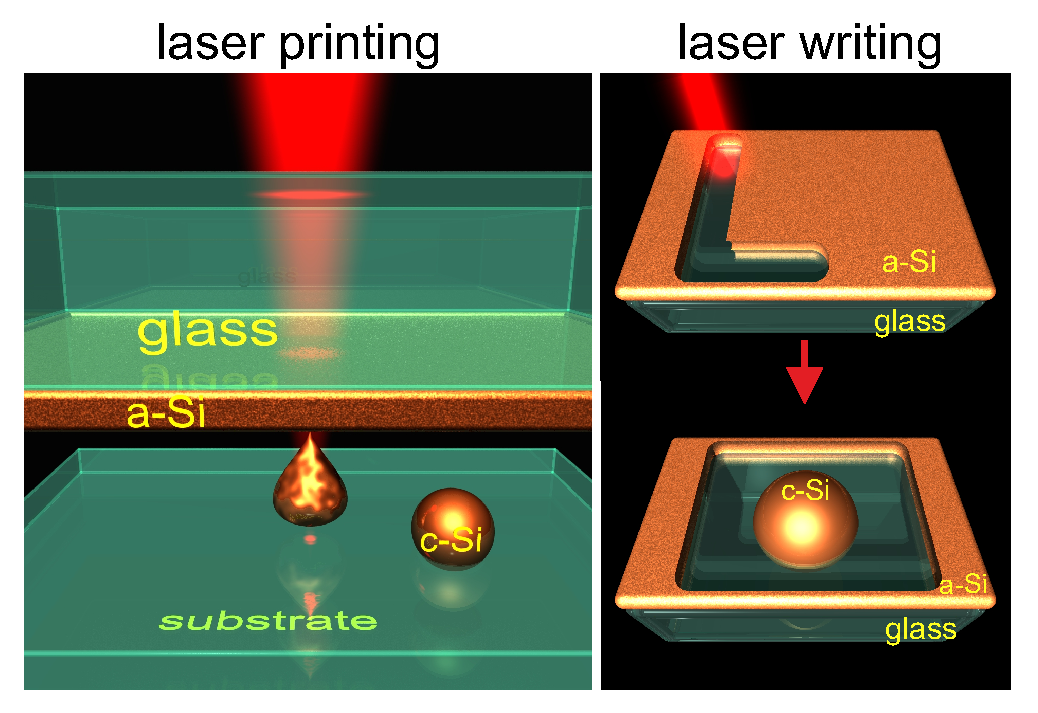
\includegraphics[width=0.5\textwidth]{figs/methods/LaserPrinting.eps}
                \end{center}
                \caption{Geometry of laser-ablation based fabrication methods of crystalline nanoparticles from amorphous
                            thin films.}
                \label{fig:LaserPrinting}
        \end{figure}

        \subsubsection{Laser Transfer of Crystalline Dielectric Particles}
        \label{met:transfer}
                Single laser pulses were selected by a Pockels cell-based pulse picker (also Avesta Project),
            focused by an oil immersion microscope objective (Olympus $100\times$)
            with a numerical aperture of $\mathit{NA}=1.4$. According to the relation $\emph{d}\approx 1.22\lambda/\mathit{NA}$, the estimated
            diameter of the beam's focal spot size was $d=0.7~\si{\upmu m}$, which was close to the value measured by a method based on
            the dependence of the laser-damaged area on incident laser energy ($0.68~\si{\upmu m}$)~\cite{liu1982simple}.
            The nanoparticles were fabricated from an $80~\si{nm}$ thick a-Si:H film deposited on a fused silica substrate by
            plasma enhanced chemical vapor deposition from a SiH$_{3}$ precursor gas.

                The nanoparticles were fabricated by single laser pulses (from a previously undamaged surface of the a-Si:H film) in a
            forward-transfer geometry, where the receiving substrate is placed under the film with a spacing
            of $\sim 50~\si{\upmu m}$ (figure~\ref{fig:LaserPrinting}(a)). This geometry has an advantage over the back-transfer geometry
            used in \cite{zywietz2014laser}, because of the possibility of transferring nanoparticles onto a wide variety of substrates,
            including opaque and structured samples.

                The silicon nanoparticles were printed at laser energies in the range of $0.5-1.2~\si{nJ}$, providing fluencies in
            the range of $0.12-0.16~\si{J/cm^{2}}$. The fabricated nanoparticles were almost spherical in shape(figure~\ref{fig:Crystallinity}(b))
            and their diameters lie in the range of $50-200~\si{nm}$, depending on the fluence.

        \subsubsection{Laser Writing of Dielectric Particles}
        \label{met:writing}
                The direct laser writing of crystalline Si nanoparticles was carried out from an initially amorphous a-Si:H film.
            The process consists of using a train of femtosecond pulses to cut patches out of the a-Si thin film\cite{makarov2016controllable,
            dmitriev2016direct}. A laser fluence $F\approx100~\si{mJ/cm^{2}}$ provides film heating close to the melting point even in a
            single shot regime, while a pulse train with a $12.5~\si{ns}$ delay between pulses leads to the temperature accumulation
            and exceeding of the ablation threshold. The heat transferring from the ablated area to the surrounding film is accumulated
            much stronger in the cut patches, which are thermally isolated from the rest of the film.
            These micro-patches are unstable at high temperatures and undergo dewetting to a certain number of similar
            nanoparticles~\cite{thompson2012solid}.

    \clearpage
    \subsection{Optical Measurements}
            All of the optical characterization measurements were carried out on a multifunctional setup, depicted in
            Fig.~\ref{fig:expSetup}. The setup allowed us to measure optical signals from single nanoparticles, provided that
            there was at least $1\mu$ m between the nanoparticle and its nearest neighbors. The XYZ-stage used for the
            positioning of the particles had $100$nm precision, giving enough control to position a single nanoparticle into
            the center of the excitation beam.

            The scattered light was collected from the top by an objective (Mitutoyo M Plan APO NIR, 100x, NA=0.7),
            sent to a Horiba LabRam HR spectrometer and projected onto a thermoelectrically cooled charge-coupled device
            (CCD, Andor DU 420A--OE 325) with a 150-g/mm diffraction grating. The spectrometer gave us a spectral resolution
            of around $1$nm.

            \begin{figure}[!ht]
                    \begin{center}
                        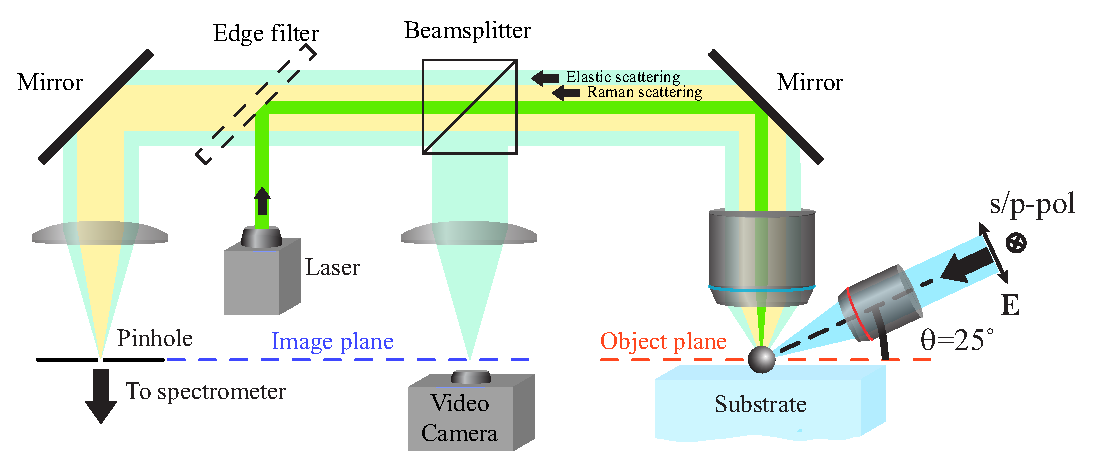
\includegraphics[width=0.9\textwidth]{figs/methods/expSetup2.eps}
                    \end{center}
                    \caption{Schematic of the experimental setup used for all of the optical measurements.}
                    \label{fig:expSetup}
            \end{figure}

        \subsubsection{Polarization-Resolved Dark-field Spectroscopy of Single Nanoparticles}
            \label{sec:Darkfield}
                For the dark-field scattering experiments, the nanoparticles were excited at an oblique angle of incidence
            (65 degrees to the surface normal) by linearly polarized light from a halogen lamp (HL--2000--FHSA)
            through a weakly-focusing objective (Mitutoyo M Plan Apo NIR, 10x, NA=0.28). The polarization allowed us to
            selectively excite different modes in the nanoparticles\cite{permyakov2015probing}, see Fig. \ref{fig:PolarizedDF}.

            \begin{figure}[!ht]
                    \begin{center}
                        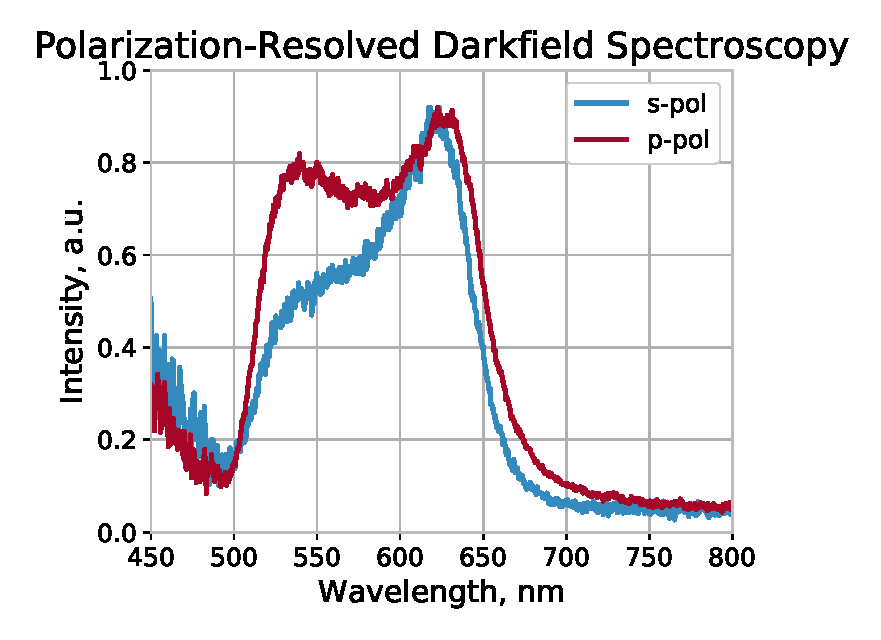
\includegraphics[width=0.6\textwidth]{figs/methods/DF/id_52780.eps}
                    \end{center}
                    \caption{Different Mie-type resonances excited by different polarizations of incident light.}
                    \label{fig:PolarizedDF}
            \end{figure}

        \subsubsection{Raman Spectroscopy of Single Nanoparticles}
        \label{sec:Raman}
                For the Raman scattering experiments, the nanoparticles were excited by one of two laser sources: a $632.8$nm HeNe laser
            or a $532$nm Nd:YAG laser, through the same channel that was used to collect the scattered light. A lowpass filter was used
            to filter out the excitation wavelength and leave only the Stokes-shifted inelastically scattered light.

                Raman intensity is proportional to the volume of the Raman-active material. One of the goals of the project was to compare
            the intensity of Raman scattering by particles with different resonance positions, which meant comparing particles of different
            sizes. This meant that for any meaningful comparison, the Raman signal had to be normalized to the volume of the particles, allowing
            comparisons of intensity per volume to be made.

    \subsection{Analytical Model of Raman Signal Enhancement by Mie resonances of Nanoparticles}
        \label{sec:Theory}
            This derivation is based on the derivation from \cite{dmitriev2016resonant}.

            To describe the enhancement of Raman scattering and analyze the role of the electric and magnetic
        Mie resonances of a silicon nanoparticle, the rigorous Green tensor approach was employed. Ideologically,
        the theoretical approach is based on earlier related studies~\cite{canccado2014theory, murphy1983enhanced}.

        In this framework, first, the spatial field distribution $\mathbf{E}_{exc}(\mathbf{r})$
        inside the nanoparticle at the excitation frequency created by an external source was determined. Assuming that a
        spherical nanoparticle in free space is illuminated by a plane wave, the normalized
        electric field inside the nanoparticle can be represented as a series of vector spherical harmonics~\cite{bohren1983absorption}:
        %
        \begin{align}
            \mathbf{E}_{exc}(\mathbf{r})=\sum\nolimits_{n=1}^\infty E_n \left(c_n\mathbf{M}_{o1n}^{(1)}(\mathbf{r}) -
            i{d_n}\mathbf{N}_{e1n}^{(1)}(\mathbf{r})\right) ,
            \label{eq1}
        \end{align}
        %
        where $c_n$ and $d_n$ are the Mie coefficients, ${{\mathbf{M}}_{o1n}^{(1)}}$ and ${{\mathbf{N}}_{e1n}^{(1)}}$ are
        the orthogonal vectorial spherical harmonics, and ${E_n} = {i^n}(2n + 1)/[n(n + 1)]$. The excitation field distribution
        at each point inside the medium defines the Raman polarization oscillating at the Stokes frequency $\omega_S$ according to
        %
        \begin{align}
            {{\bf{P}}_s}\left( {\bf{r}} \right) = {\chi _s}\hat \alpha_j \left( {\bf{r}} \right){{\bf{E}}_{exc}}\left( {\bf{r}} \right),
            \label{eq2}
        \end{align}
        %
        where $\chi_s$ is the scalar Raman susceptibility, and $\hat \alpha_j$ is the Raman polarizability tensor representing
        the threefold degenerate transverse optical (TO) phonon mode excitation~\cite{ralston1970spontaneous, peter2010fundamentals}.
        Induced Raman polarization, in turn, produces an electromagnetic field at the observation point
        $\mathbf{r}_0$ given by $\mathbf{E}_s(\mathbf{r}_0) = (\omega_s^2/c^2)\int\limits_V {{{\hat G}_s}\left( {{{\mathbf{r}}_0},{\mathbf{r}}} \right){{\mathbf{P}}_s}\left( {\mathbf{r}} \right){d^3}{\mathbf{r}}}$,
        where  ${\hat G_s}\left( {{{\mathbf{r}}_0},{\mathbf{r}}} \right)$ is the Green tensor at the Stokes frequency accounting
        for the Si nanoparticle and integration is carried out over the nanoparticle volume $V$. Finally, the collected signal at
        the point $\mathbf{r}_0$ is presented in the form:
        %
        \begin{align} %Final collected signal
            S\left( {{{\mathbf{r}}_0}} \right)
                =  \sum\limits_j {\left \langle{{\mathbf{E}}_s^*\left( {{{\mathbf{r}}_0}} \right){{\mathbf{E}}_s}\left( {{{\mathbf{r}}_0}} \right)} \right\rangle}
                = \sum\limits_j {\frac{{\omega _s^4}}{{{c^4}}}\iint\limits_V {{d^3}{{\mathbf{r}}_1}{d^3}{{\mathbf{r}}_2}\left\langle {\hat G_s^*\left( {{{\mathbf{r}}_0},{{\mathbf{r}}_1}} \right){\mathbf{P}}_s^*\left( {{{\mathbf{r}}_1}} \right){{\hat G}_s}\left( {{{\mathbf{r}}_0},{{\mathbf{r}}_2}} \right){{\mathbf{P}}_s}\left( {{{\mathbf{r}}_2}} \right)} \right\rangle }}  \\
                = \sum\limits_j {\frac{{\omega _s^4}}{{{c^4}}}\iint\limits_V {{d^3}{{\mathbf{r}}_1}{d^3}{{\mathbf{r}}_2}\hat G_s^*\left( {{{\mathbf{r}}_0},{{\mathbf{r}}_1}} \right){\mathbf{E}}_{exc}^*\left( {{{\mathbf{r}}_1}} \right){{\hat G}_s}\left( {{{\mathbf{r}}_0},{{\mathbf{r}}_2}} \right){{\mathbf{E}}_{exc}}\left( {{{\mathbf{r}}_2}} \right)\chi _s^2\left\langle {\hat \alpha _j^*\left( {{{\mathbf{r}}_1}} \right) \otimes {{\hat \alpha }_j}\left( {{{\mathbf{r}}_2}} \right)} \right\rangle }},
            \label{eq4}
        \end{align}
        %
        where summation is performed over the three degenerate TO phonon modes. Since the Raman scattering is a spontaneous process
        (until we enter the stimulated Raman scattering regime), the  induced polarization $\mathbf{P}_s$ is not coherent across
        the whole particle. Therefore, in Eq.~(\ref{eq4}), the averaging is carried out over all possible realizations of the Raman
        polarization $\mathbf{P}_s$. Taking into account that the correlation length of the Raman scattering in silicon $L_c$ is of
        the order of tens nanometer and much less than the nanoparticle diameter, the correlation of the Raman
        polarizability tensors can be approximated by the Dirac delta function
        $\left\langle {\hat \alpha_j \left( {{{\mathbf{r}}_1}} \right) \otimes \hat \alpha_j \left( {{{\mathbf{r}}_2}} \right)} \right\rangle \sim \delta \left({{\mathbf{r}_1} - {\mathbf{r}_2}} \right)$.
        Under this assumption, Eq.~(\ref{eq4}) reduces to
        %
        \begin{align}
            S\left( {{{\bf{r}}_0}} \right) = \frac{{\omega _s^4}}{{{c^4}}}\sum\limits_j {\int\limits_V {{d^3}{\bf{r}}{{\left| {{{\hat G}_s}\left(
            {{{\bf{r}}_0},{\bf{r}}} \right){{\hat \alpha }_j}{\chi _s}{{\bf{E}}_{exc}}\left( {\bf{r}} \right)} \right|}^2}} }
            \label{eq5}
        \end{align}
        %
        \begin{figure}[h!]
            \begin{center}
                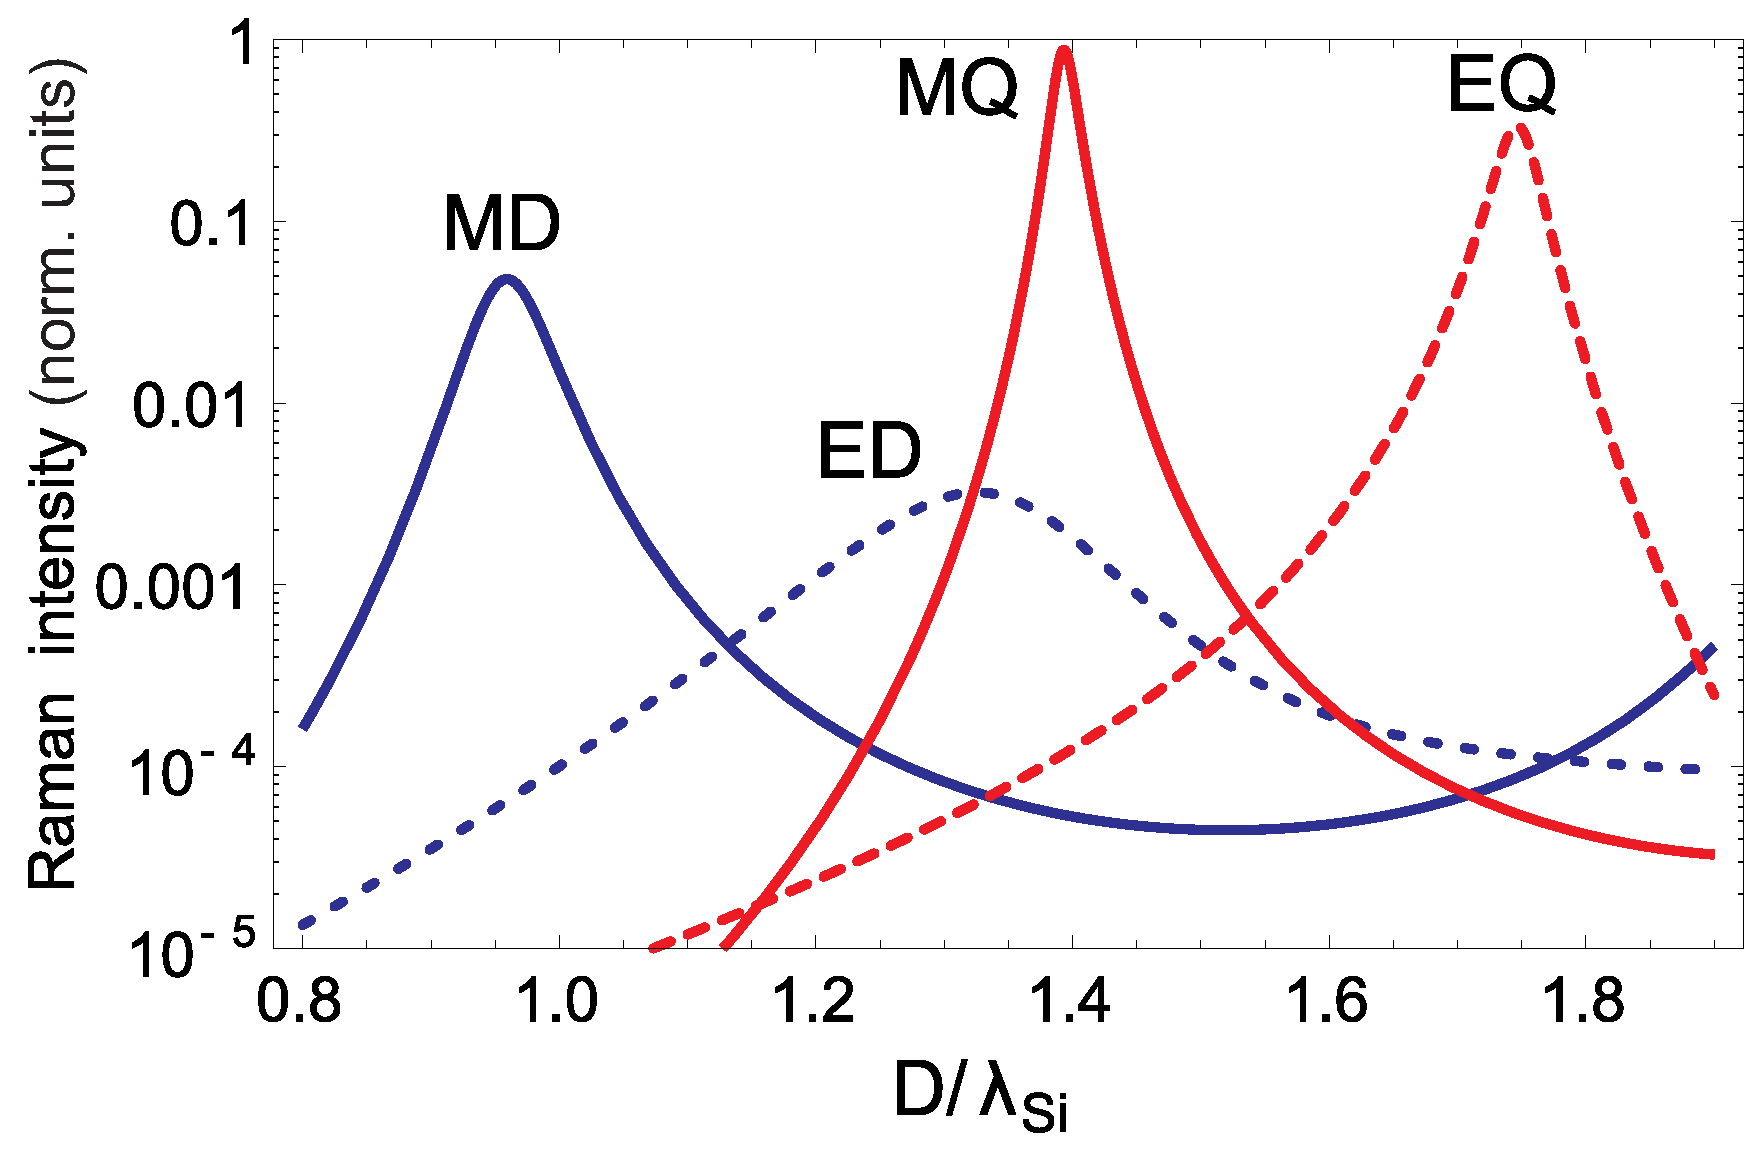
\includegraphics[width=0.5\textwidth]{figs/intro/TheoryEnhancement.eps}
            \end{center}
            \caption{Log plot of normalized intensity of Raman scattering as a function of dimensionless nanoparticle diameter for the magnetic dipole (MD),
            electric dipole (ED), magnetic quadrupole (MQ) and electric quadrupole (EQ) resonances.}
            \label{fig:TheoryEnhancement}
        \end{figure}

            Expression~(\ref{eq5}) can be simplified with the use of the single-mode approximation. The
        electromagnetic response of an optically small Si nanoparticle at the excitation wavelength is dominated by a single
        magnetic or electric multipole resonance depending on the particle radius~\cite{evlyukhin2010optical}. Therefore,
        only one resonant term in Eq.~(\ref{eq1}) is required and the electric field inside the nanoparticle can be represented as ${
        {\mathbf{{E}}}_{exc}} \approx {E_n}{c_n}{\mathbf{M}}_{o1n}^{(1)}$, for the $n-$th magnetic resonance, and
        ${{\mathbf{{E}}}_{exc}}\approx -i{E_n}{d_n}{\mathbf{N}}_{e1n}^{(1)}$, for the $n-$th electric resonance.
        Furthermore, since the Raman shift in silicon is small compared to the linewidth $\gamma$ of
        Mie resonance at $\omega_0$, the main contribution to the Green tensor is provided by the same eigenmode of
        the system. Therefore, expanding the Green tensor in the series of eigenmodes~\cite{ishimaru1991electromagnetic} and keeping only
        the resonant term:
        %
        \begin{align}
            {\hat G_s}\left( {{{\bf{r}}_0},{\bf{r}}} \right) \approx \frac{{{c^2}}}{{{N^2}}}\frac{{{\bf{u}}\left( {{{\bf{r}}_0}} \right) \otimes
            {\bf{u}}^*\left( {\bf{r}} \right)}}{{{{\left( {{\omega _0} + i\gamma } \right)}^2} - \omega _s^2}},
            \label{eq8}
        \end{align}
        %
        where ${{\mathbf{u}}\left( {{\mathbf r}} \right)}$ is the spatial field distribution of the eigenmode, and
        ${N^2} = {\int {{\mathop{\rm Re}\nolimits} \varepsilon \left( {\bf{r}} \right)\left| {{\bf{u}}\left( {\bf{r}} \right)} \right|} ^2}{d^3}{\bf{r}}$
        is the normalization constant. Finally, integrating the expression (5) over the whole volume $V$ of the nanoparticle,
        the following simple expression, describing the Raman signal enhanced by a single Mie resonance, can be written:
        %
        \begin{align}
            S\left( {{{\mathbf{r}}_0}} \right) \approx V{\left( {\frac{{{\omega _s}}}{c}} \right)^4}{\left| {\frac{{{\chi_s s_n}}}{{{{\left( {{\omega
            _0} + i\gamma } \right)}^2} - \omega _s^2}}} \right|^2},
            \label{eq9}
        \end{align}
        %
        where $s_n$ stands for the Mie coefficient, either $c_n$ or $d_n$ of the corresponding mode. The above expression clearly
        shows that the total enhancement of Raman scattering depends on two factors: the enhancement of the excitation field
        inside the medium, and the Purcell enhancement of the Raman dipoles radiation~\cite{checoury2010deterministic}.

        The two key parameters entering Eq.~(\ref{eq9}) are the resonance frequency $\omega_0$ and the resonance linewidth $\gamma$.
        The resonance frequency can be easily estimated numerically, while for the estimation of the resonance linewidth one can
        employ analytical expressions from Ref.~\cite{lai1991effect}. Substituting these values into Eq.~(\ref{eq9}), one can obtain the desired
        spectrum of Raman scattering enhanced by the resonances of a silicon sphere. This spectrum (normalized by the particle
        volume $V=4\pi R^3/3$) is plotted in Fig.~\ref{fig:TheoryEnhancement} as a  function of dimensionless nanoparticle diameter $D/\lambda_{\rm Si}$
        with $\lambda_{\rm Si}=163$~nm being the wavelength of the excitation signal inside the silicon for the magnetic dipole (MD), electric dipole (ED),
        magnetic quadrupole (MQ) and electric quadrupole (EQ) resonances assuming a constant excitation wavelength of 633~nm,
        used below in experiments.

        The derived single-mode expression (\ref{eq9}) makes it possible to clearly separate contributions of each Mie resonance of the
        nanoparticle into the total Raman scattering enhancement. As follows from Fig.~(\ref{fig:TheoryEnhancement}), the strongest enhancement
        is associated with the MQ resonance due to its high $Q-$factor. Notably, the predicted Raman scattering enhancement
        at the MD resonance, which occurs for the smallest particles, is more than an order of magnitude larger than that for
        the ED resonance.


    \subsubsection{Numerical Methods}
    \label{sec:Numeric}
        Several numerical methods were used to simulate the scattering properties of the fabricated nanoparticles~--- to prove their
        crystalline phase, to probe their shape, to determine their size. The initial idea was to use the Discrete Dipole Approximation,
        because it is very flexible and can work with scatterers of arbitrary geometry. The main problem that was encountered was the fact
        the method is very involved (especially if one tries to incorporate substrate interaction), and computationally intensive for
        the required problems. Many calculations turned out to be excessive~-- a simple Mie theory calculation,
        while simulating a slightly different geometry, was more than enough to model the required parameters, with error well within the
        requirements.

        For calculations of field distribution inside the nanoparticles presented in this thesis, CST Microwave Studio was used.
        It is an  EM simulation package that uses the Finite Integration Technique for most of its calculations.

        \subsubsection{Discrete Dipole Approximation}
        \label{subsec:DDA}

                For the DDA calculations, a custom, Python-based implementation was written, PyDDA~--- a reimplementation of an existing
            Matlab toolkit, DDA-SI\cite{loke2011discrete}. The implementation even included surface-interaction components in its' calculations,
            but the complexity of the calculation and difficulty of accurately modeling particles led to the DDA being abandoned in favor of plain
            Mie theory, which provided more than enough accuracy for the purposes of the project.

            \begin{figure}[h!]
                \centering
                \begin{subfigure}[b]{0.3\textwidth}
                    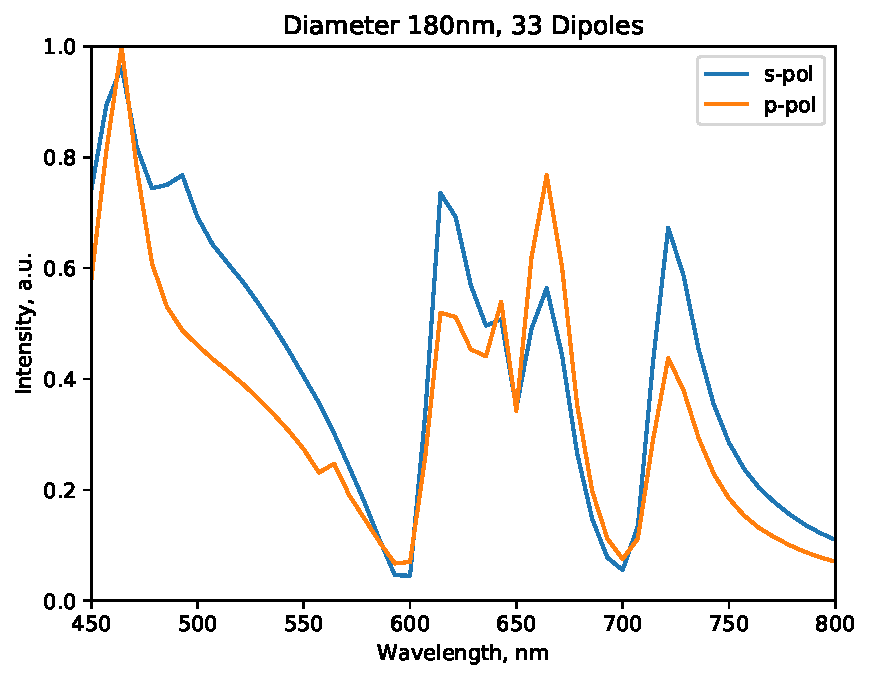
\includegraphics[width=\textwidth]{figs/methods/DDA/n_33.pdf}
                    \caption{}
                \end{subfigure}~
                \begin{subfigure}[b]{0.3\textwidth}
                    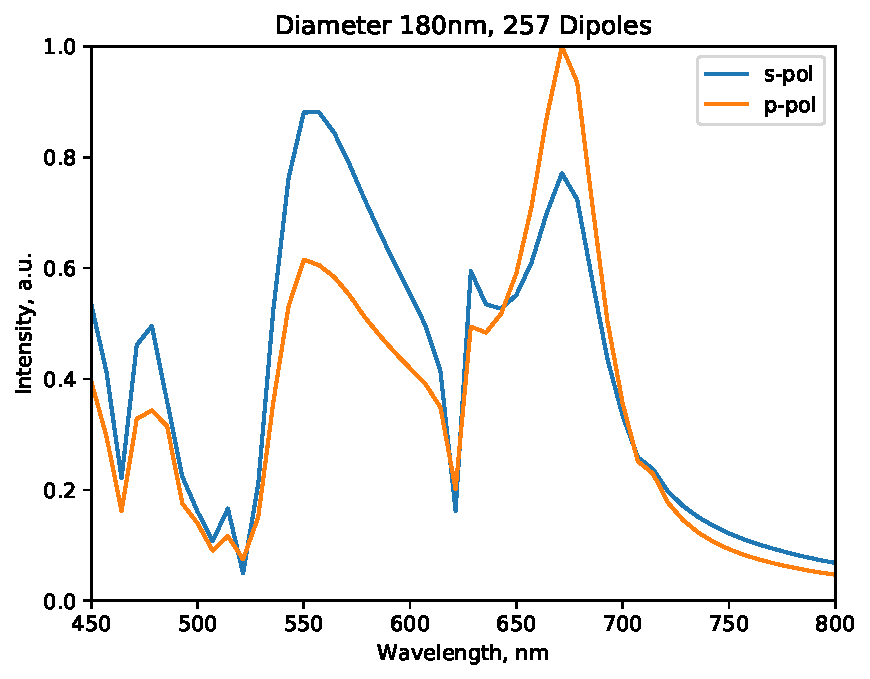
\includegraphics[width=\textwidth]{figs/methods/DDA/n_257.pdf}
                    \caption{}
                \end{subfigure}~
                \begin{subfigure}[b]{0.3\textwidth}
                    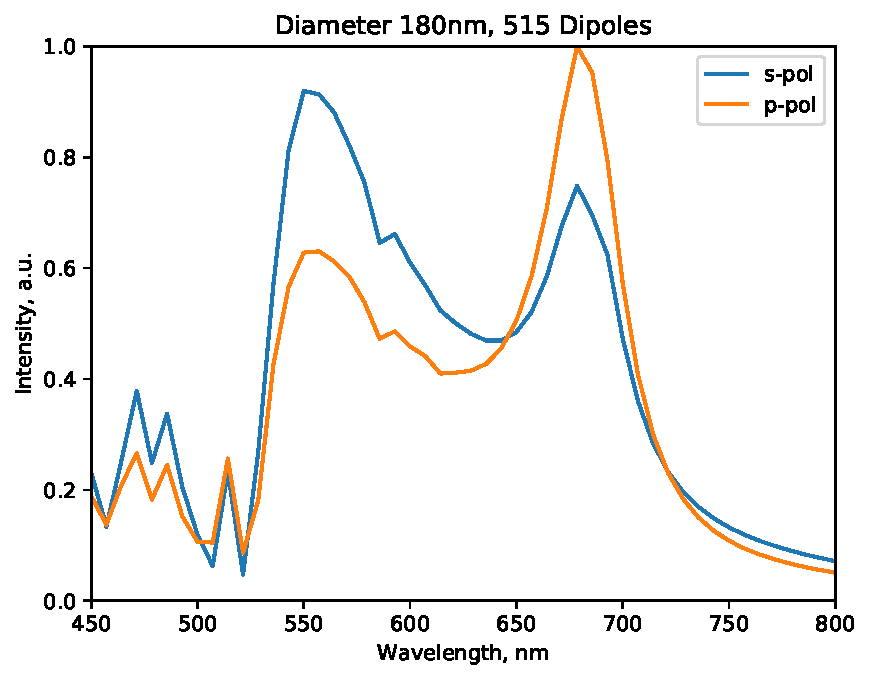
\includegraphics[width=\textwidth]{figs/methods/DDA/n_515.pdf}
                    \caption{}
                \end{subfigure}
                \caption{Scattering from isotropic sphere modeled by DDA using a) 33, b) 257, c) 515 dipoles to model the sphere.}
                \label{fig:DDA_Dipole}
            \end{figure}

        \clearpage
        \subsubsection{Finite Integration Technique}
        \label{subsec:FIT}

                CST Microwave studio was used to model field distribution inside and around the silicon nanoparticles, to
            demonstrate the electric field confinement at different types of resonances (electric and magnetic dipole resonances).
            The model was a slightly oblate spheroid, corresponding to the experimentally determined geometric parameters of the
            nanoparticles.

            \begin{figure}[!ht]
                \centering
                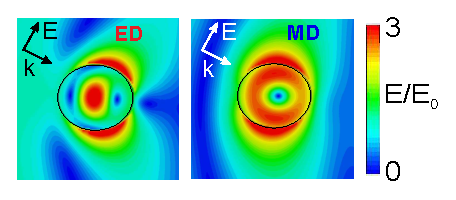
\includegraphics[width=0.7\textwidth]{figs/methods/FIT/CST.eps}
                \caption{Field distribution inside 180nm spheroid nanoparticle with 1.12 oblateness parameter at electric and magnetic dipole resonances,
                    calculated using CST Microwave Studio}
                \label{fig:CST}
            \end{figure}

\clearpage

% !TeX spellcheck = english
% !TEX root = thesis.tex
\section{Experimental Results}
    \subsection{Fabrication of Crystalline Silicon Nanoparticles}
        \label{sec:Fabrication}

        \subsubsection{Laser Writing of Nanoparticles}

            \begin{figure}[!ht]
                    \begin{center}
                        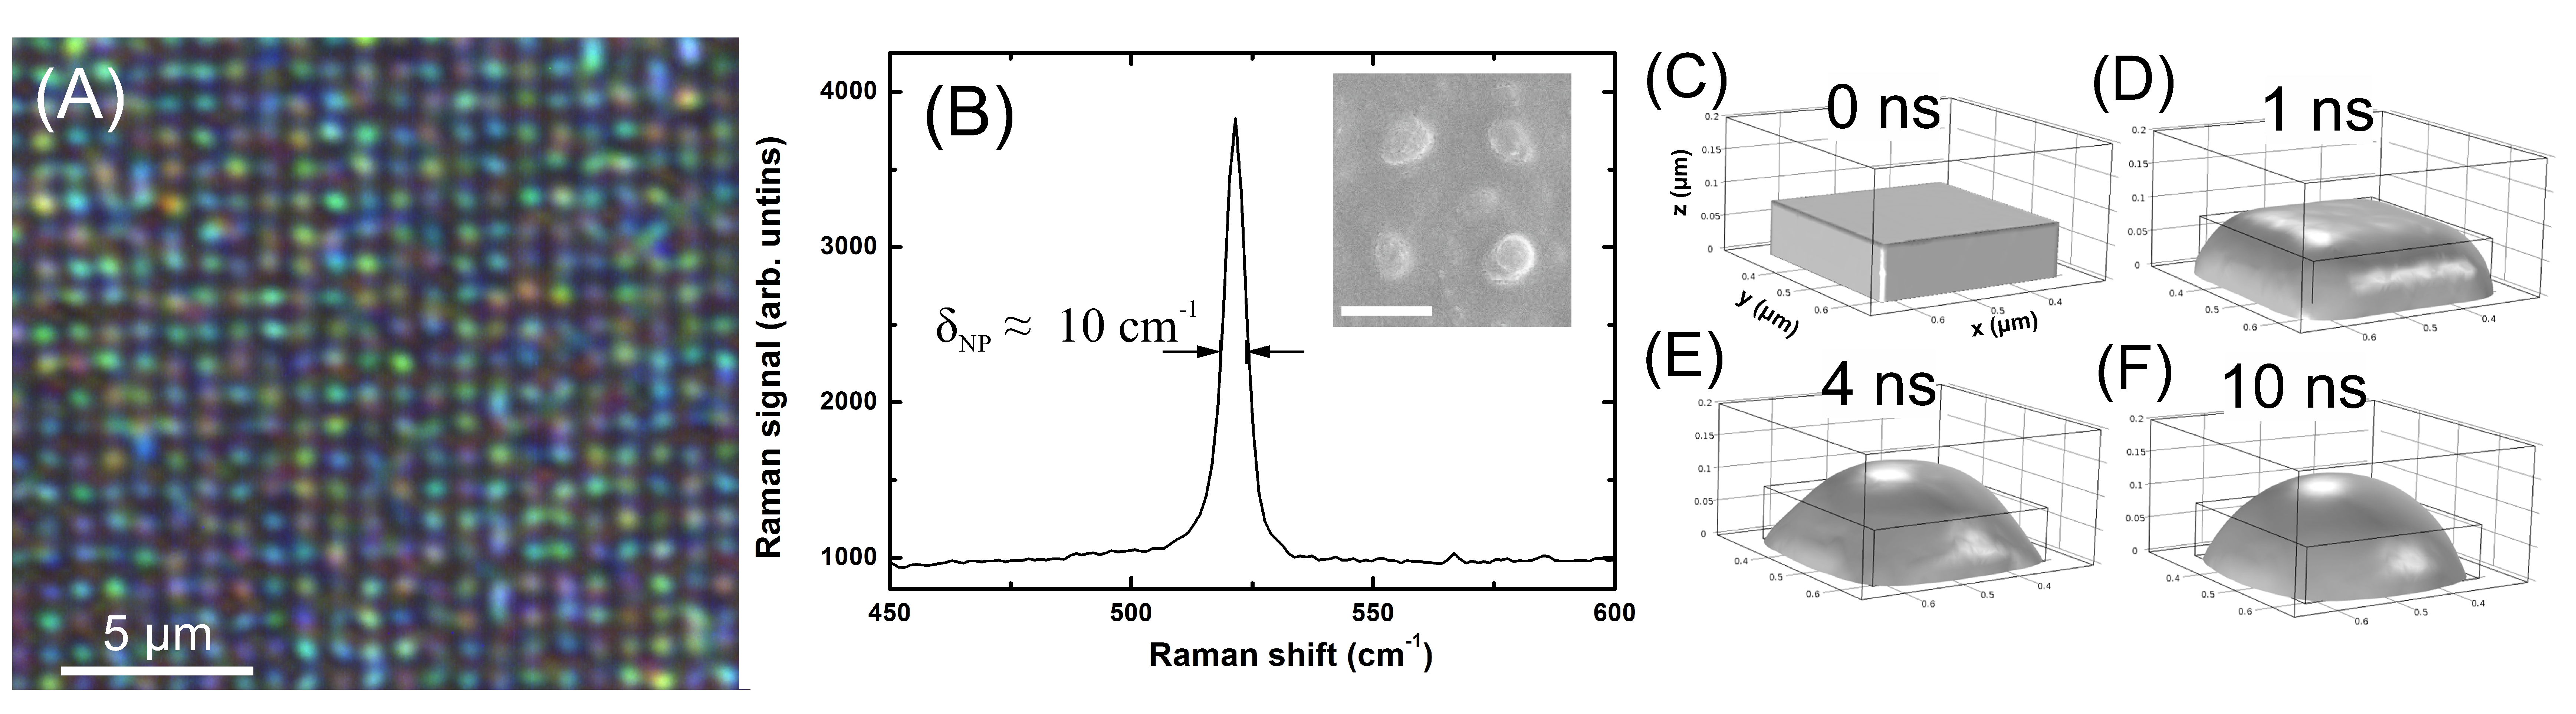
\includegraphics[width=0.9\textwidth]{figs/results/fab/LaserWriting.eps}
                    \end{center}
                    \caption{A. Dark-field image of array of nanoparticles fabricated by direct laser writing. B. Raman peak of single nanoparticle. Inset - SEM image
                    of several nanoparticles. C-F. COMSOL Model of transformation of liquid silicon patch into hemisphere.}
                    \label{fig:LaserWriting}
            \end{figure}

                Under the optimal conditions of fabrication, the method described in Sec.~\ref{met:writing}
            can create and ordered array of nanoparticles, with a period of 0.9~$\mu$m. Dark-field imaging of the arrays show that
            the nanoparticles exhibit bright colors, which indicates resonant scattering~--- see Fig.~\ref{fig:LaserWriting}A.
            The cutting process produces square patches, but the resulting arrays are arrays of nearly circular nanoparticles, as can be
            seen on SEM images~--- see Fig.~\ref{fig:LaserWriting}B. This is caused by the dewetting of the thermally isolated patches into
            hemispherical particles, caused be heat accumulation and overheating during the cutting process. COMSOL Simulations of a
            square liquid silicon patch with a side of 300~nm and height of 80~nm on a substrate of fused silica, solving the incompressible
            Navier-Stokes equations with realistic models of the materials show, that after about ten nanoseconds, the the initial patch has
            transformed into an hemisphere with an approximate height and width of 140~nm and 350~nm~--- see Figs.~\ref{fig:LaserWriting}C-F.
            This is in good qualitative agreement with the experimentally observed nanoparticles.

                Measurement of Raman signals from these nanoparticles shows that the particles are, indeed, crystalline~---  they demonstrate
            a narrow peak at 520~cm$^{-1}$, with a half-width of about 10~cm$^{-1}$ (Fig.~\ref{fig:LaserWriting}B).
            This half-width correspond to average crystallite sizes of less than 10~nm, according to previous studies~\cite{campbell1986effects}.

        \subsubsection{Laser Transfer of Nanoparticles}
            \begin{figure}[!ht]
                    \begin{center}
                        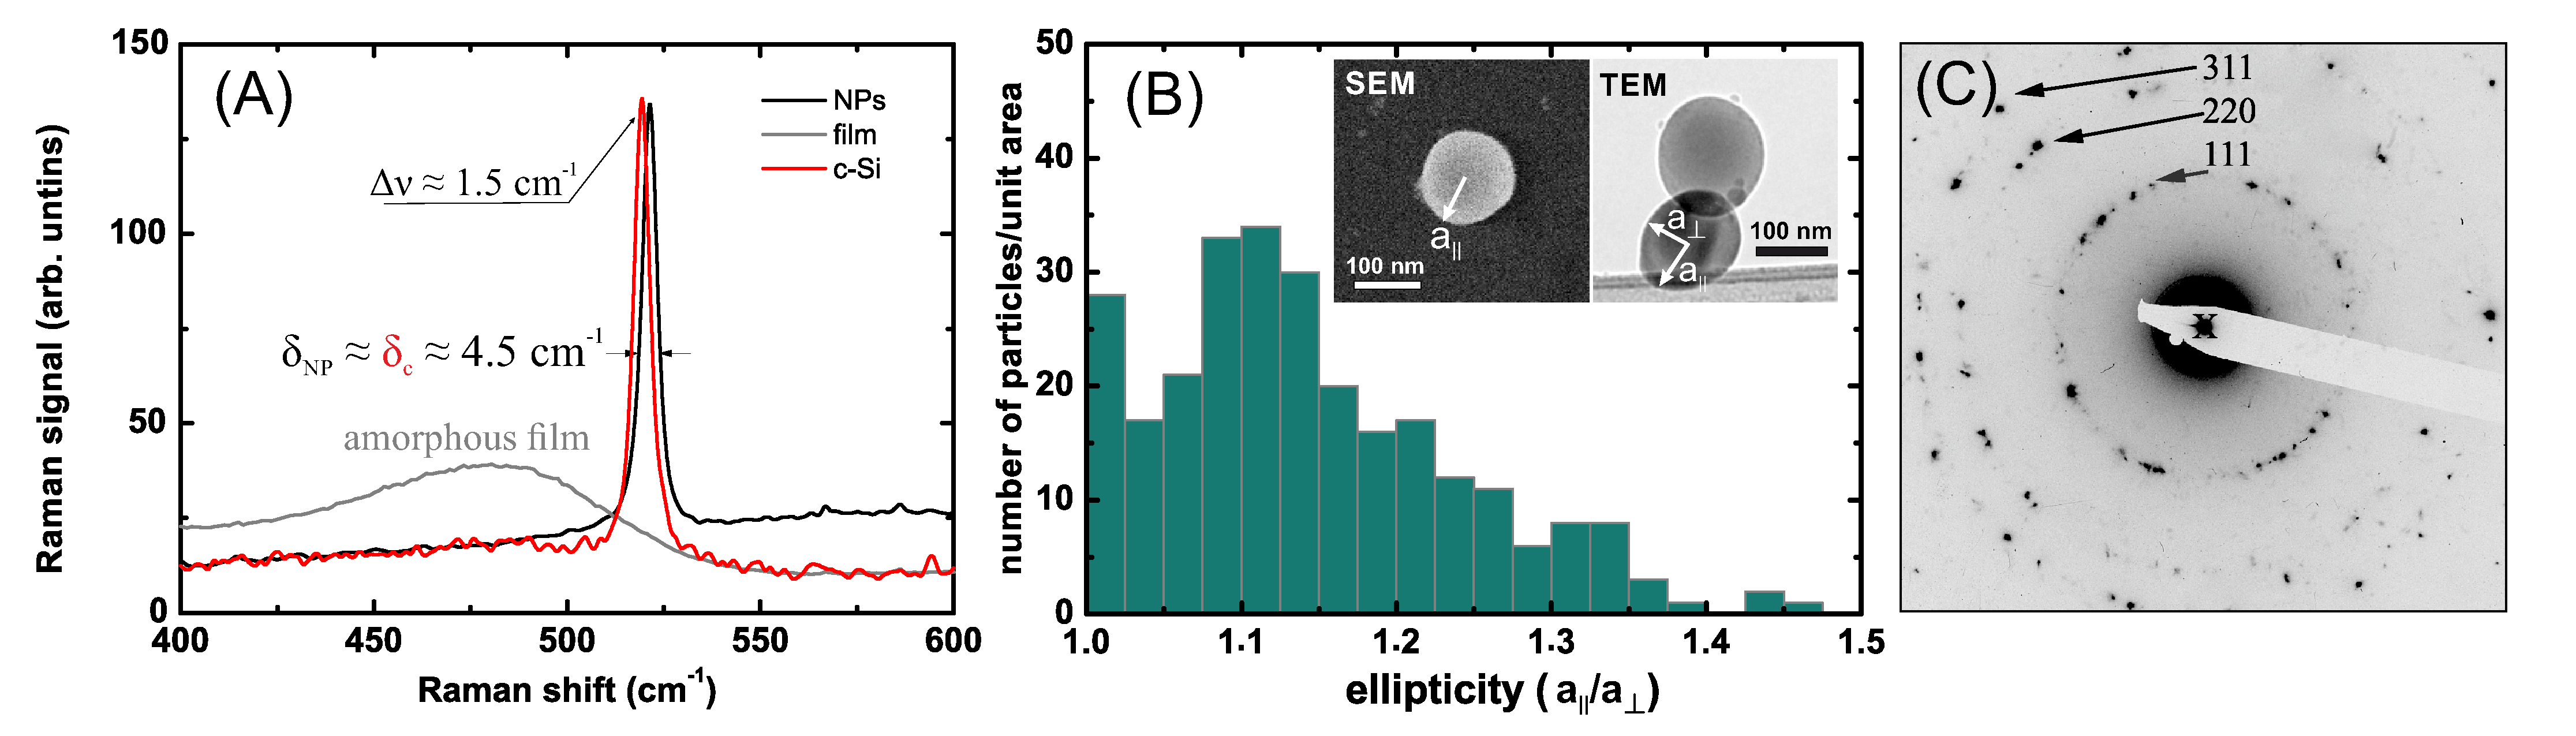
\includegraphics[width=0.9\textwidth]{figs/results/fab/Crystallinity.eps}
                    \end{center}
                    \caption{A. Raman signal from (gray) initial amorphous film, (red) bulk crystalline silicon, (black) single nanoparticle,
                    fabricated by laser transfer. B. Histogram of ellipticity of nanoparticles; insets~--- SEM and TEM images of nanoparticles. C.
                    Electron diffraction pattern from cluster of nanoparticles.}
                    \label{fig:Crystallinity}
            \end{figure}


                The initial a-Si:H film, used for the fabrication of the nanoparticles was amorphous, a fact supported by its broad Raman peak,
            centered at 480~cm$^{-1}$. In contrast to the Raman signal of the initial film, the Raman signal from the individual nanoparticles,
            fabricated using the laser transfer method described in Sec.~\ref{met:transfer}, had narrow peaks centered at 521.5~cm$^{-1}$, which
            is very close to the reference Raman signal from a bulk crystalline silicon wafer, centered at 520~cm$^{-1}$. The slight positive shift
            of the position of the Raman peak from the nanoparticles, $\Delta$$\nu$ = 1.5~cm$^{-1}$, can be explained by residual compressive stress
            ~\cite{de1996micro} in the nanoparticles, from the transfer process from donor to acceptor substrate. Similar to the previous method,
            by measuring the half-width of the Raman peak of the nanoparticles, around 4--5~cm$^{-1}$, one can estimate the minimum crystallite size,
            which, in this case is larger than $\sim$20~nm, because the Raman peaks of the nanoparticles have
            almost the same half-width as the peak from a bulk crystalline silicon wafer (4.5~cm$^{-1}$) ~\cite{campbell1986effects}.

                The Raman measurements are supported with electron diffraction patterns of clusters of the printed nanoparticles. The fabricated nanoparticles
            were deposited on transmission electron microscopy specimen grids (3-mm-diameter, 200-mesh copper grids, coated on one side with a 20-nm-thick
            film of amorphous carbon). Using TEM, along with electron diffraction to demonstrate the crystallinity, the size and shape and composition
            of the nanoparticles were studied, using bright and dark-field TEM imaging, see Fig.~\ref{fig:Crystallinity}B.
                The electron diffraction pattern from a cluster of nanoparticles shows a number of clear maxima, which correspond to several crystalline planes
            if silicon (Fig.~\ref{fig:Crystallinity}C). Because the specimen grids were even, the particles were deposited at different angles to the substrate,
            allowing their shapes to be studied from the TEM images~--- providing information on the particles' oblateness. The average ellipticity
            of the particles, $a_{\parallel}/a_{\perp}\approx$1.12, where $a_{\parallel}$($a_{\perp}$) is the particle semi-major
            (semi-minor) axis oriented parallel (perpendicular) to the surface of the substrate. Scanning electron microscopy, (SEM, using a Carl Zeiss Neon 40),
            of particles deposited on an flat, even substrate, confirm that the particles possess axial symmetry along the substrate
            normal (Fig.~\ref{fig:Crystallinity}B). These results correlate with previously observed ellipticity of the printed silicon
            nanoparticles~\cite{zywietz2014laser}.

                Previous studies of femtosecond laser ablation as a method of fabricating silicon nanoparticles~\cite{zywietz2014laser, zywietz2014generation}
            have shown that the average size of the fabricated nanoparticles is determined by the laser fluence used. Experiments carried
            out as part of this thesis also showed similar behavior. The experiments demonstrated two distinct regimes of nanoparticle
            fabrication. The first regime, observed at fluencies of up to 150~mJ/cm$^{2}$, has nanoparticle size proportional to the laser
            fluence, which can be seen in Fig.~\ref{fig:Darkfield}A--C as a change in color from blue to red. This can be explained by the
            spallation mechanism of laser ablation, where a thin molten layer is spalled due to the laser-induced tensile pressure waves~\cite{ionin2013thermal,wu2014microscopic},
            breaking into a number of liquid droplets via the Rayleigh-Plateau instability~\cite{papageorgiou1995breakup}.
            The photomechanically spalled volume increases as $V\sim\ln(E)$ when illuminated by a Gaussian beam, because of the
            logarithmic dependence of the spalled surface layer area $r^{2}_{s}\sim\ln(E)$~\cite{bauerle2013laser}, while
            the thickness of the layer remains almost constant~\cite{ionin2013thermal} or even slightly decreases~\cite{wu2014microscopic}.
            Previous studies of nanoparticle fabrication from crystalline silicon an increase of the molten volume led
            to an increase in the number~\cite{zywietz2014generation} and size~\cite{zywietz2014laser}of fabricated nanoparticles,
            which agrees with current results (Fig.~\ref{fig:Darkfield}A--C).

                The second regime of nanoparticle fabrication is observed at fluencies over ~150~mJ/cm$^{2}$, generating large (red) and
            small nanoparticles at the same time, with a broad size distribution~---- see Fig.~\ref{fig:Darkfield}D. This regime is caused
            by the unstable boiling of superheated silicon~\cite{bulgakova2001pulsed, ionin2013thermal, wu2014microscopic}. In this regime,
            nanoparticles are formed by explosive decomposition of material into small droplets and vapor~\cite{itina2009molecular,wu2014microscopic},
            which result in nanoparticles with average sizes less than 100~nm~\cite{amoruso2004generation}. This regime has been extensively
            studied~\cite{amoruso2004generation, tull2006formation} for biomedical applications. The high-fluence regime (Fig.~\ref{fig:Darkfield}D)
            does not produce monodisperse, reproducible nanoparticles, unlike the low low-fluence regimes (Fig.~\ref{fig:Darkfield}A--C). This
            makes the low-fluence regimes more desirable for controllable nanoparticle fabrication and deposition onto acceptor substrates.
            Raman, TEM and SEM characterization of the printed silicon nanoparticles were used to quantify their crystalline phase,
            proving that it is possible to controllably fabricate crystalline silicon nanoparticles from amorphous films with a single stage
            process.

    \subsection{Characterization of Resonant Optical Modes of the Nanoparticles}
        \label{sec:DarkfieldExp}

        \begin{figure}[!ht]
                \begin{center}
                    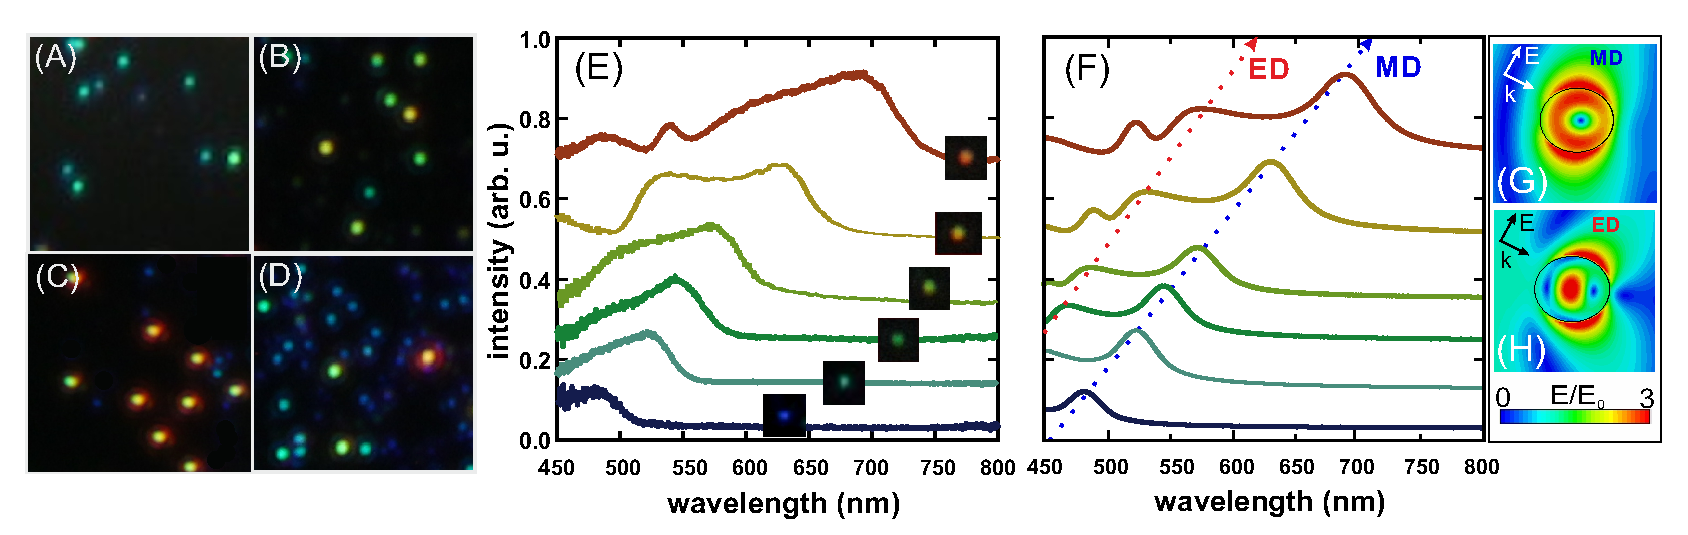
\includegraphics[width=0.9\textwidth]{figs/results/char/DarkField.eps}
                \end{center}
                \caption{Dark-field optical images of silicon nanoparticles fabricated at different peak fluencies:
                120 (A), 130 (B), 140 (C), 160~mJ/cm$^{2}$ (D). Experimental (E) and theoretical (F) spectra for
                scattered p-polarized incident light (angle of incidence is 65$^{\circ}$) from individual nanoparticles
                with the radius parallel to substrate surface a$_{\parallel}$ = 55~nm (blue), 65~nm (spring green),
                68~nm (green), 72~nm (olive), 85~nm (yellow) and 92~nm (red) with the ellipticity coefficient of 1.12.
                Numerically calculated electric field distributions in the silicon nanoparticle with a$_{\perp}$ = 85~nm
                 the wavelengths of 635~nm (G) and 525~nm (H).}
                \label{fig:Darkfield}
        \end{figure}

            Dark-field scattering measurements showed that the nanoparticles posses a number of resonances, corresponding to different
        Mie-type resonances, see Fig.~\ref{fig:Darkfield}. To determine which resonances correspond to electric dipole (ED) and
        magnetic dipole (MD) resonances, the scattering properties of and electric field distribution near and inside the nanoparticles were
        modeling using the FIT technique in CST Microwave Studio.

            The scattering geometry was modeled as a c-Si ellipsoid with different axis
        ($a_{\perp}$ and $a_{||}$) and the fixed ellipticity $a_{\parallel}/a_{\perp}\approx$~1.12, i.e. for
        the most probable ellipticity parameter in the experiments. The ellipsoid was irradiated by a plane wave
        at the angle 65$^{\circ}$ in vacuum, modeling the geometry used in the dark-field scattering experiments. Substrate effects
        were deemed to be insignificant, which is justified in the next section. The optical properties for
        c-Si were taken from Ref.~\cite{vuye1993temperature}. Modeling of scattering spectra (Fig.~\ref{fig:Darkfield}F) showed good agreement
        with the corresponding experimental ones (Fig.~\ref{fig:Darkfield}E), whereas the modeled electric field distributions
        in the ellipsoids at different wavelengths proved the excitation of MD (Fig.~\ref{fig:Darkfield}G) and ED (Fig.~\ref{fig:Darkfield}H).

    \subsection{Determining Size of Nanoparticle from Optical Resonance Positions}

        \begin{figure}[!ht]
                \begin{center}
                    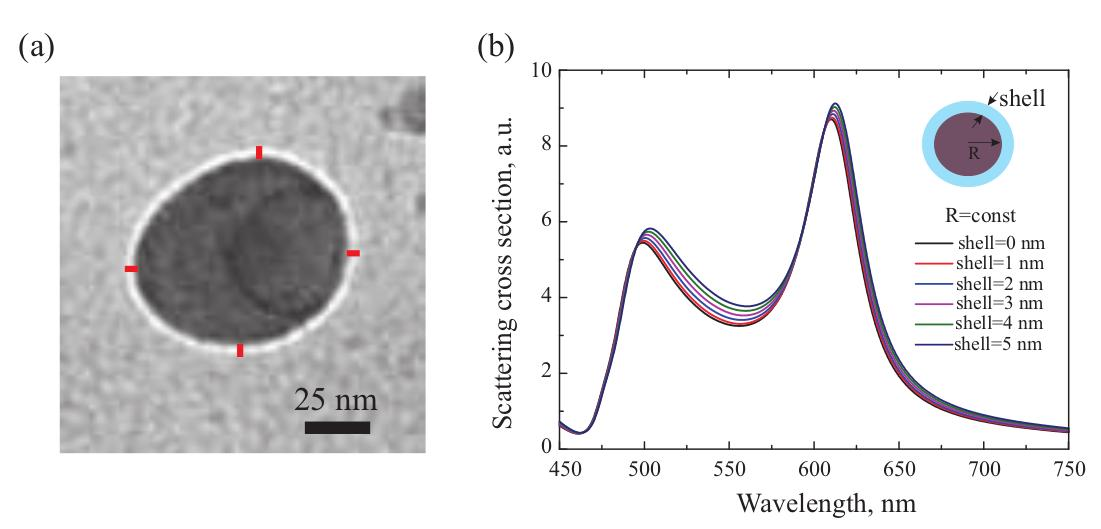
\includegraphics[width=0.9\textwidth]{figs/results/char/CoreShell.jpg}
                \end{center}
                \caption{\textbf{a}. TEM image of the typical silicon nanoparticle fabricated using laser-induced
                            forward transfer technique. Red lines represent 5 nm. \textbf{b}. Total scattering cross sections of
                            silicon nanoparticle (R = 75 nm) coated with silica layers with different thicknesses.}
                \label{fig:CoreShell}
        \end{figure}

        Resonant optical properties of silicon nanoparticles are known to be sensitive to their shape~\cite{zywietz2015electromagnetic},
        crystallinity~\cite{zywietz2015electromagnetic,dmitriev2016laser}, to the substrate~\cite{miroshnichenko2015substrate} and
        to the thickness of native oxide layer~\cite{zywietz2015electromagnetic, fu2012directional},
        which is always present on silicon surface~\cite{morita1990growth}. The shape of the particles was characterized using
        SEM and TEM measurements, while the diameter of silicon core has been extracted from dark-field spectroscopy experiments, by
        comparing the positions of the experimental resonances to those of Mie resonators of different sizes.

        Additional experimental measurements and numerical simulations were done to analyze the influence of native silicon oxide layer
        on the optical properties of the studied nanoparticles. The average thickness of the native oxide layer was
        estimated by transmission electron microscopy (TEM) of a typical silicon nanoparticle, see Fig.~\ref{fig:CoreShell}A.
        The measurements showed that nanoparticles are coated with a thin layer of SiO$_2$, at most 5-nm-thick, which agrees
        with previous results~\cite{zywietz2015electromagnetic, fu2012directional}.
        To analyze the influence of the oxide layer on the resonant properties of nanoparticles,
        total scattering cross section spectra of a crystalline silicon nanoparticle (D = 150 nm) surrounded by
        silica shells with different thicknesses were simulated, see Fig.~\ref{fig:CoreShell}. For the sake of simplicity, the simulations have been carried out
        using Mie theory~\cite{bohren1983absorption}. The results of the simulations confirm that in the case of a fixed silicon core diameter, the appearance of an additional
        5-nm-thick silica layer leads to red spectral shifts of both electric and magnetic dipole resonances of the
        nanoparticle at most by $≈ 4.2$nm and $≈ 2.5$nm. The influence of different substrates has been analyzed in
        Ref.~\cite{miroshnichenko2015substrate} The authors have demonstrated that both electric and magnetic dipole resonances of
        crystalline silicon nanoparticle
        placed on the fused silica substrate exhibit small red spectral shifts with respect to the resonances of the nanoparticle
        in free space. In the case of nanoparticle with the diameter of $D = 130 $nm these shifts are around $≈ 3.5 $nm and $≈ 0.5$ nm.
        Therefore, the spectral shift of the nanoparticle’s magnetic dipole resonance is almost insensitive to both
        the substrate and the native silica layer. This allows for accurate estimation of the the diameter of silicon core of the nanoparticle
        from the spectral position of magnetic dipole resonance in the dark-field spectroscopy measurements by
        comparing to the simulations based on Mie theory.


    \subsection{Raman Scattering Enhancement from Single Nanoparticles}
        \label{sec:RamanExp}

        \begin{figure}[!ht]
            \begin{center}
                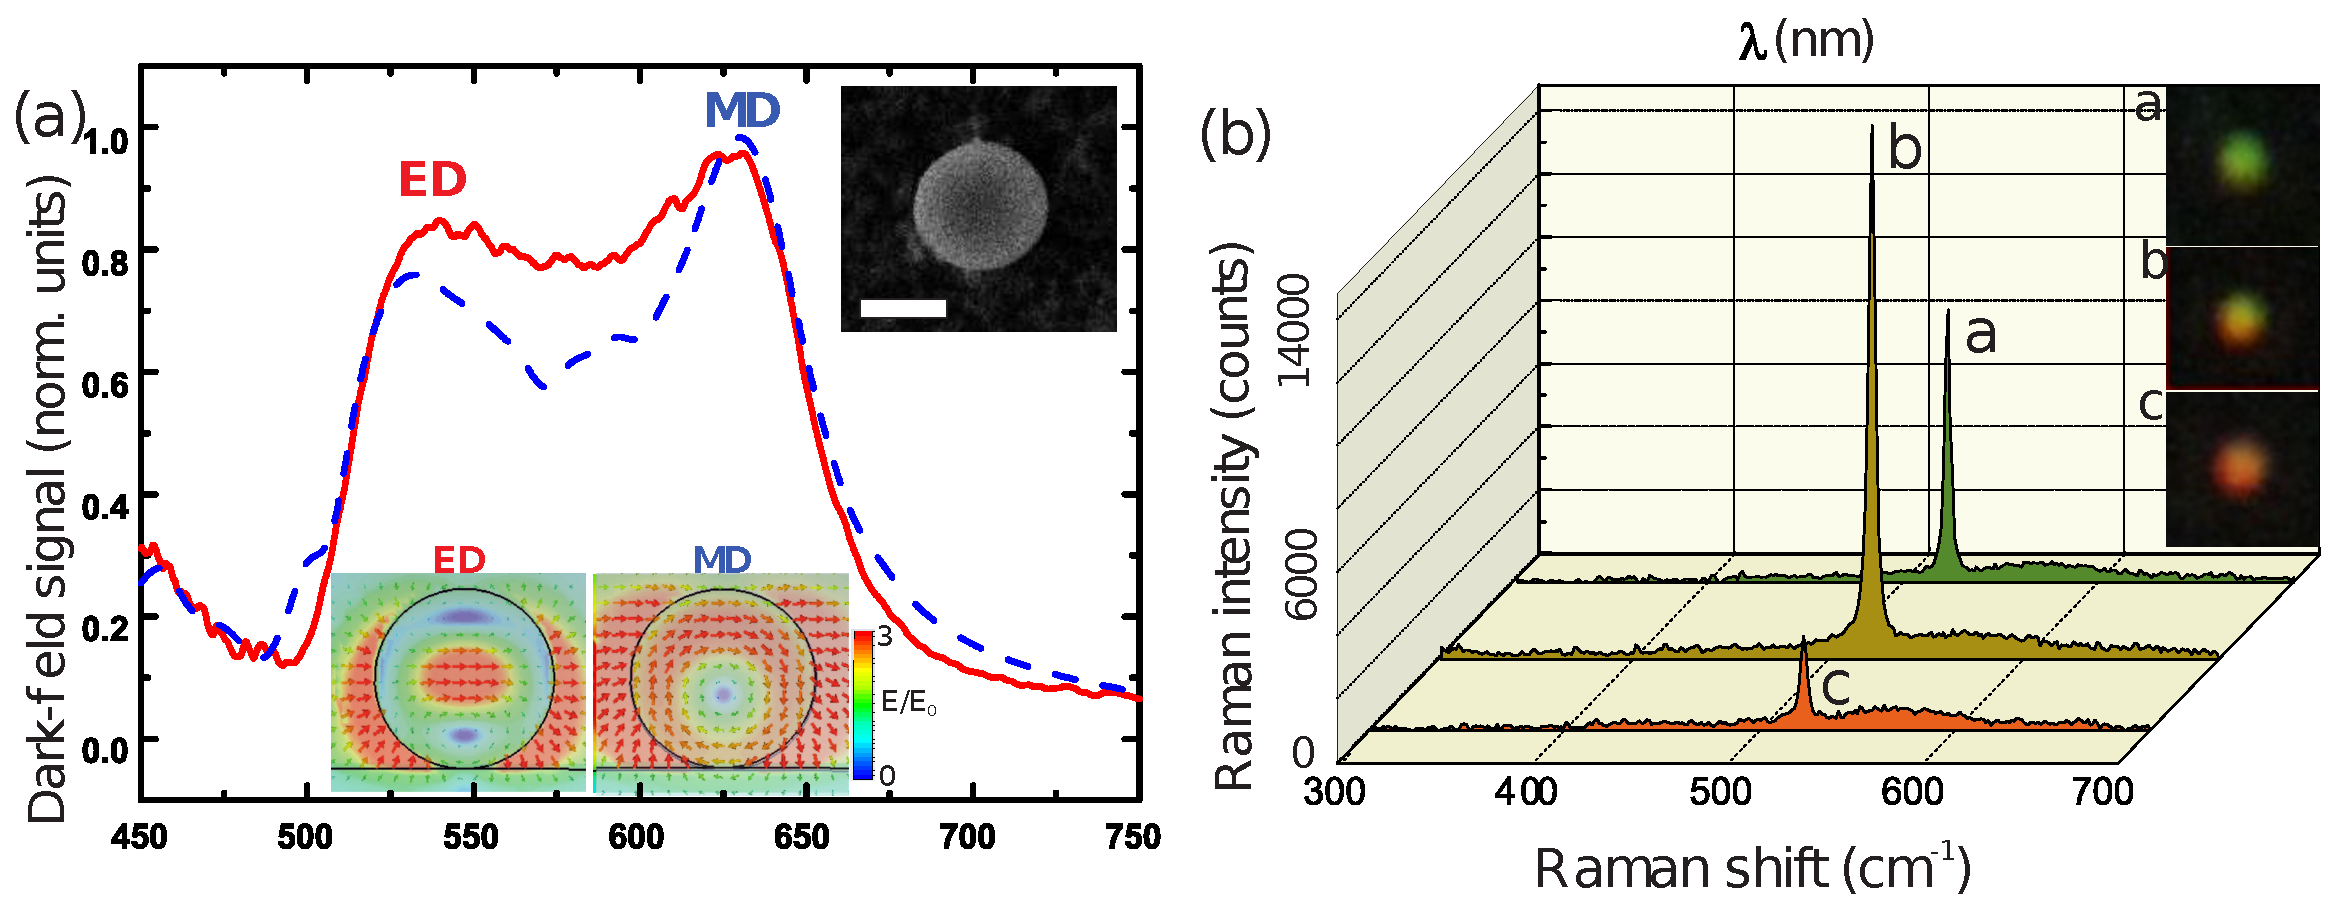
\includegraphics[width=0.9\textwidth]{figs/results/enhance/EnhancementExperiment.eps}
            \end{center}
            \caption{(\textbf{a}) Experimental (solid) and theoretical (dashed) scattering spectra for s-polarized incident light.
            Bottom inset: the electric field distribution at different wavelengths, corresponding to electric dipole (ED) and magnetic
            dipole (MD) resonances. Upper inset: SEM image of typical ablative c-Si nanoparticle (scale bar represents 100~nm). (\textbf{b})
            Raman spectra for different nanoparticles at the excitation wavelength of 633 nm and the corresponding dark-field optical images of the
            nanoparticles: (a) D=153 nm, (b) D=158 nm, (c) D=173 nm.}
            \label{fig:EnhancementExp}
        \end{figure}


            Theoretically predicted Raman scattering enhancement on different Mie-type resonances, see Sec.~\ref{sec:Theory} was demonstrated
        experimentally be measuring Raman scattering from single crystalline nanoparticles, fabricated using the laser transfer process described
        in Sec.~\ref{met:transfer}. During the Raman measurements it was noted that different nanoparticles exhibit different intensities of
        Raman scattering, and that that intensity of the scattering has a non-trivial dependence on particle size, see Fig.~\ref{fig:EnhancementExp}b.
        For the excitation wavelength of $\lambda$=633~nm, the maximum Raman intensity corresponds to particles with a diameter $D\approx 155$~nm,
        which corresponds to a magnetic dipole (MD) resonance at the excitation wavelength. To be able to compare different Raman measurements among
        themselves they needed to be normalized, because Raman scattering is dependent on the volume of the excited Raman-active medium. To calculate
        enhancement factors, a baseline intensity also needed to be chosen. A non-resonant particle, e.g. with diameter $D\approx$135~nm, demonstrating
        the smallest measured Raman signal,
        was chosen as the baseline intensity, relative to which the enhancement factor was calculated. The enhancement factor, EF, was
        calculated according to the formula EF~=~(I/I$_{\rm norm}$)$\times$(V/V$_{\rm norm}$), where I is Raman
        scattering signal from a studied nanoparticle with known diameter and volume V, I$_{\rm norm}$ is Raman signal from
        a nanoparticle of known volume V$_{\rm norm}$ chosen as the baseline, in this case, a nanoparticle with the smallest Raman signal.
        The maximum value of the enhancement factor (EF) for nanoparticles with a MD resonance at 633nm was calculated to be $EF\approx$140.

        \begin{figure}[!hb]
            \begin{center}
                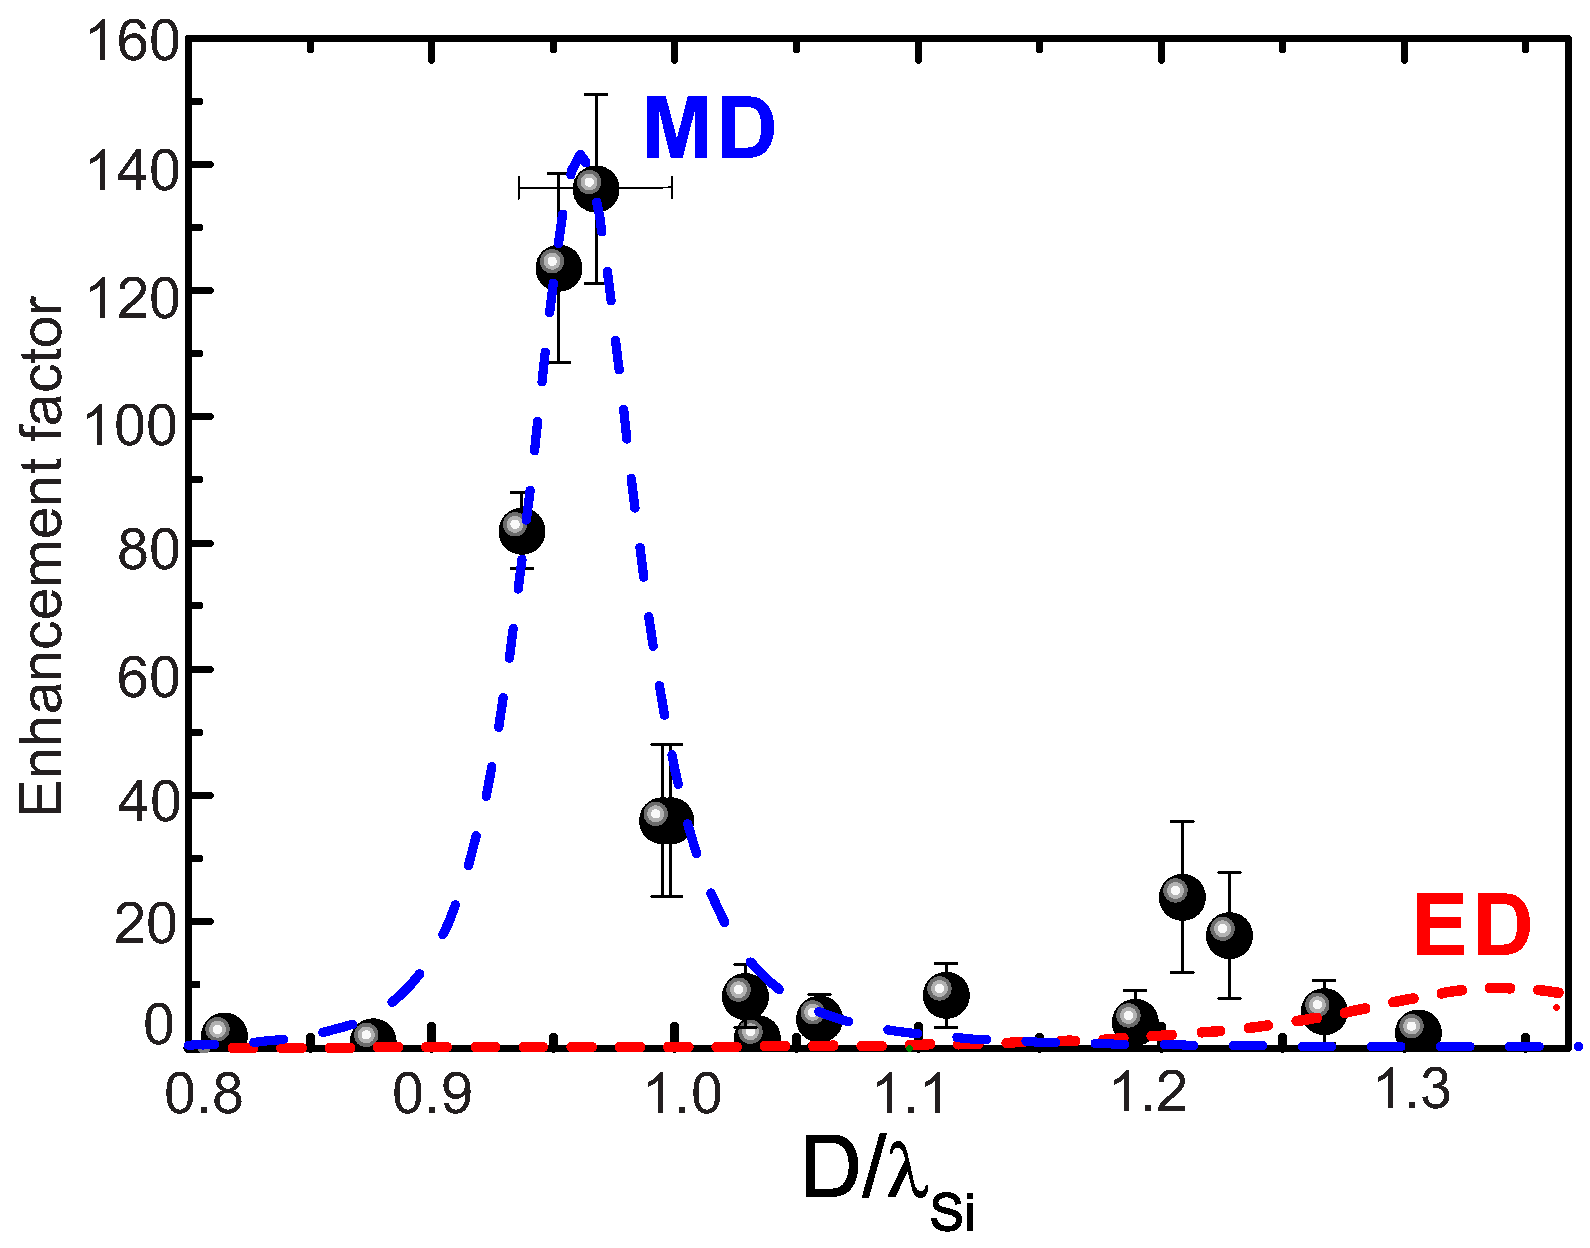
\includegraphics[width=0.5\textwidth]{figs/results/enhance/EnhancementExperimentTheory.eps}
            \end{center}
            \caption{Theoretical (dashed curves) and experimental (black dots) dependencies of the enhancement factor for Raman
            scattering from spherical silicon nanoparticles on their diameter D normalized to the excitation wavelength in silicon.
            Theoretical dependence consists of two contributions from magnetic dipole (blue dashed curve) and electric dipole
            (red dashed curve).}
            \label{fig:EnhancementExpTheory}
        \end{figure}

            In order to compare the experimental enhancement factors to the predicted contributions from different resonances, the
        enhancement factor of Raman scattering needed to be plotted relative to the dimensionless particle size $D/\lambda_{\rm Si}$,
        taking into account the dispersion of the refractive index of silicon. The result of this is show on Fig.~\ref{fig:EnhancementExpTheory}.
        The resulting dependence has a pronounced peak at D/$\lambda_{\rm Si}$ $\approx$ 1, with $EF\approx$140 i.e. near the
        magnetic dipole resonance, which agrees with the theoretical prediction from Sec.~\ref{sec:Theory}. This maximum EF is about 5-7 times larger than the EF for the
        electric dipole. Insets in Fig.~\ref{fig:EnhancementExp}a, showing the confinement of the electric field at the ED and MD resonances
        provide an illustrative interpretation of this enhancement. The MD resonance confines a larger fraction of the electric field inside the
        nanoparticle than the ED resonance, therefore producing more efficient excitation of the Raman active medium and thus increasing total
        Raman polarization and emission. The theoretical predictions, for perfect spherical nanoparticles, have an even larger difference in EF
        between ED and MD resonances ($\sim$ 10), which is not achieved in experiment because of nanoscale imperfections in the nanoparticles
        and the existence of a thin native oxide layer~\cite{fu2012directional, zywietz2015electromagnetic}.
        The results shown in Fig.~\ref{fig:EnhancementExpTheory} are limited to nanoparticle diameters $D/\lambda_{\rm Si}<1.3$
        because the fabrication method is limited in the maximum size of produced nanoparticles without significant deviations from a spherical shape.
        Even a small deviation from the spherical leads to suppression of the MQ resonance~\cite{fu2012directional}, which makes large but aspherical
        particles applicable to only study enhancement on ED and MD resonances.

% !TeX spellcheck = english
% !TEX root = thesis.tex
\section*{Results}
        Two methods of fabricating crystalline nanoparticles, based on femtosecond laser ablation, nanoparticles were developed.
    A direct laser-writing technique, allowing for precise patterning of a substrate (coated with a thin film of $\alpha$-Si),
    where a train of femto-second laser pulses is used to pattern a thin film of $\alpha$-Si~--- cutting it into isolated patches
    of silicon, which dewet into nanoparticles from the absorbed heat from the pulses. With precise optimization of the thickness
    of the film, the laser fluence and pulse frequency, it is possible to create ordered arrays of nearly identical nanoparticles.
    The second technique, forward transfer of nanoparticles by single femtosecond laser pulses from an amorphous thin film onto
    a acceptor substrate, is more flexible~--- particle diameter can be controlled in the range of $100-200$nm by adjusting the
    fluence of the laser pulses, there is virtually no limitation on the type of acceptor substrate, i.e. almost anything can be coated
    by crystalline nanoparticles. Both methods produce crystalline nanoparticles in a single-step process, making the fabrication
    methods very simple and potentially high throughput.

    It has also been shown, both theoretically and experimentally, that Raman scattering from the crystalline silicon nanoparticles
    can be enhanced by the Mie-type modes of the nanoparticles. This happens when the wavelength of the excitation source corresponds
    to the wavelength of a Mie resonance of the nanoparticle. The enhancement happens because of field confinement inside the nanoparticle,
    leading to more efficient excitation of the Raman-active volume of crystalline silicon.
    The strongest enhancement has been shown to be from magnetic resonances, because of the strong field confinement inside the particle
    and high Q factor of the resonance.
    $140$-fold increase in Raman scattering from resonant particles, enhanced on the magnetic dipole resonance has been demonstrated.

    \clearpage
    The main results of the project can be summarized as follows:
    \begin{enumerate}
        \item Two methods for single-stage fabrication of crystalline silicon nanoparticles using femto-second laser ablation were developed:
            \begin{itemize}
                \item Direct laser writing of arrays of nanoparticles in an amorphous silicon thin-film;
                \item Forward laser transfer of crystalline nanoparticles from amorphous silicon thing-films to arbitrary substrates.
            \end{itemize}
        \item The crystallinity of the nanoparticles was confirmed by electron diffraction and Raman measurements.
        \item The implemented DDA model was applied for apsherical nanoparticles.  The shape-dependent shifts of resonances
                obtained from the model were compared to pure Mie-theory and FIT modeling.
        \item The elasting scattering of light from nanoparticles was measured in a dark-field configuration.
        \item The obtained spectral positions of Mie-type resonances allowed to estimate sizes of nanoparticles.
        \item Measurements of Raman scattering intensity from crystalline nanoparticles were carried out.
        \item It was shown the Raman signal intensity demosntrates resonant beahviour with change of
                relative positions of excitation wavelength and Mie-type resonances of the nanoparticles.
    \end{enumerate}

        The results of the project were published in two papers the peer-reviewed journal Nanoscale: ``Laser fabrication of
    crystalline silicon nanoresonators from an amorphous film for low-loss all-dielectric nanophotonics''~\citeA{dmitriev2016laser} and
    ``Resonant Raman scattering from silicon nanoparticles enhanced by magnetic response''~\citeA{dmitriev2016resonant} and in
    three conference proceedings: ``Femtosecond laser transfer of silicon nanoparticles with enhanced Raman response''~\citeA{dmitriev2016femtosecond},
    ``Single-stage fabrication of low-loss dielectric nanoresonators from high-loss material''~\citeA{dmitriev2016single},
    ``Direct Femtosecond Laser Writing of Optical Nanoresonators''~\citeA{dmitriev2016direct}.

\clearpage

% !TeX spellcheck = english
% !TEX root = thesis.tex
\section*{Acknowledgements}

        I would like to thank D. Baranov for developing the theoretical description of the processes studied in this project.

        I would like to thank V. Milichko and my supervisor, A. Samusev, for helping with designing, optimizing and carrying the experimental work:
    Dark-field spectroscopy and Raman scattering.

        I would like to thank I. Mukhin for carrying out SEM experiments needed for this project.

        I would like to thank A. Sitnikova for carrying out TEM and X-Ray diffractometry experiments needed for this project.

        I would also like to S. Makarov for the huge amount of assistance he provided throughout the whole project~--- help with
    designing and building and optimizing the fabrication setup, assitance with numerical simulations and detailed discussions about the
    physics of the underlying processes in the fabrication techniques.


\clearpage

\appendix
% !TeX spellcheck = english
% !TEX root = thesis.tex
\section{Mie Scattering of Light}
\label{ap:Mie}
    An important problem for dielectric nanophotonics is the scattering of electromagnetic radiation by
    a homogeneous sphere. This problem has an analytical solution, generally called Mie theory\cite{mie1908beitrage}. The following
    is a condensed version of the solution, following the presentation from Ref. \cite{ng2000manipulation}.
    We will assume an x-polarized incident wave with amplitude $E_0$, propagation constant $\beta_0$ traveling in the $z$ direction:

    \begin{align}
        \vec{E}_{inc} = E_0 e^{i\beta_0z}\hat{x}
    \end{align}

    \subsection{Maxwell's Equations}
        Starting with
        \begin{align}
            \nabla \times \vec{E} &= i\omega\mu\vec{H} \\
            \nabla \times \vec{H} &= -i\omega\epsilon\vec{E}
        \end{align}

        Taking the rotor of the equations and substituting,

        \begin{align}
            \nabla \times (\nabla \times \vec{E}) &= i\omega\mu \nabla \vec{H} = \omega^2 \epsilon\mu\vec{E} \\
            \nabla \times (\nabla \times \vec{H}) &= i\omega\epsilon \nabla \vec{E} = \omega^2 \epsilon\mu\vec{H}
        \end{align}

        Applying the vector identity,

        \begin{align}
            \nabla \times \nabla \vec{A} = \nabla (\nabla \cdot \vec{A}) - \nabla \cdot (\nabla\vec{A})
        \end{align}

        We get the following wave equations

        \begin{align}
            \nabla^2\vec{E} + k^2_m\vec{E} &= 0 \label{mie:waveE}\\
            \nabla^2\vec{H} + k^2_m\vec{H} &= 0 \label{mie:waveH}\\
            k^2_m &= \omega^2\epsilon\mu \label{mie:kvec}
        \end{align}

        With $k_m$ as the wave vector in the surrounding medium. The final aim of this derivation is to get vector solutions
        of the wave equations. We begin by
        \begin{itemize}
            \item Transitioning to a spherical coordinate system ${r, \theta, \phi}$, since our system is spherically symmetrical
            \item Defining a scalar function $\psi_{l,m}$
            \item Defining a constant vector $\vec{r}$
        \end{itemize}

        The scalar function will be a solution of
        \begin{align}
            \nabla^2\psi + k^2_m\psi = 0 \label{mie:scalar}
        \end{align}

        We can construct three vector solutions:

        \begin{align}
            \vec{L} &= \nabla\psi_{l,m} \\
            \vec{M}_{l,m} &= \nabla\times\vec{r}\psi_{l,m} \\
            \vec{N}_{l,m} &= \frac{1}{k_m}\nabla\times\vec{M}_{l,m}
        \end{align}

        All solutions satisfy the wave equations. $\vec{N}_{l,m}$ and $\vec{M}_{l,m}$ are solenoidal functions and are rotors of each other,
        like $\vec{H}$ and $\vec{E}$. $\vec{L}$, on the other hand is purely longitudinal, so we omit it in this analysis.

    \subsection{Scalar Solution}

        In spherical coordinates, the scalar solution, $\psi_{l,m}$ of Equation \ref{mie:scalar} is a function of ${R, \theta, \phi}$
        \begin{align}
            \frac{1}{r^2}\frac{\partial}{\partial r}\left(r^2\frac{\partial\psi}{\partial r}\right)
                + \frac{1}{r^2\sin(\theta)}\frac{\partial}{\partial\theta}\left(\sin(\theta\frac{\partial\psi}{\partial\theta})\right)
                + \frac{1}{r^2\sin^2(\theta)}\frac{\partial^2\psi}{\partial\phi^2} + k^2_m\psi = 0
        \end{align}

        Next, we seek a solutions that separates the variables:

        \begin{align}
            \psi(r,\theta,\phi) &= R(r)\Theta(\theta)\Phi(\phi)
        \end{align}

        Defining constants $m, Q$, we separate the components into separate solutions:

        \begin{align}
            \frac{d^2\Phi}{d\phi^2} + m^2\Phi &= 0 \\
            (1 - \cos^2(\theta))\frac{d^2\Theta}{d(\cos(\theta))^2} - 2\cos(\theta)\frac{d\Theta}{d(\cos(\theta))}
                + (Q - \frac{p^2}{1-cos^2(\theta)}) &= 0 \\
            r^2\frac{d^2R}{dr^2} + 2r\frac{dR}{dr} + (k^2_mr^2 - Q^2)R &= 0
        \end{align}

        The solutions to these equations are as follows:

        For $\Phi$
        \begin{align}
            \Phi = e^{\pm i m \phi}
        \end{align}

        For $\Theta$, representing it as an associated Legendre equation:
        \begin{align}
            Q &= l(l+1) \rightarrow \\
            \Theta &= P^m_l(\nu) = \frac{(1-\nu^2)^{\frac{m}{2}}}{2^l l!}\frac{d^{l+m}(\nu^2-1)^l}{d(\nu)^{l+m}} \\
            \nu &= \cos(\theta)
        \end{align}

        From now on, $P_l^m = P_l^m(\nu)$.

        And for $R$
        \begin{align}
            R &= \sqrt{\frac{2}{\pi}}Z_l(p) \\
            p &= k_m r
        \end{align}

        Where $Z_l(p)$ represents the radial spherical Bessel $j_l(p)$ or first order Hankel $h_l(p)$. $h_l(p)$, being infinite in
        the far field are used to represent an outgoing spherical wave pattern for the scattered field. $j_l(p)$ is finite in the
        origin, so it is a correct representation of incident and transmitted fields.

        Combining all of these,

        \begin{align}
            \psi_{l,m}(r, \theta, \phi) = \sqrt{\frac{1}{\pi}}Z_l(k_m r)P_l^m e^{im\phi}
        \end{align}

        or, separating into even and odd components:

        \begin{align}
            \psi_{l,m,\substack{e\\ o}}(r, \theta, \phi) = \sqrt{\frac{1}{\pi}}Z_l(k_m r)P_l^m \substack{\cos\\\sin}(m\phi)
        \end{align}

    \subsection{Vector Solution}

        Using the previous equation,

        \begin{align}
            \vec{M}_{l,m, \substack{e \\ o}} &= \nabla \times \hat{r}(r \psi_{l, m, \substack{e \\ o }})\\
            \vec{r} &= \hat{r}r
        \end{align}

        By applying the rotor:

        \begin{align}
            \vec{M}_{l,m}(\hat{r}) &= 0 \\
            \vec{M}_{l,m, \substack{e \\ o}} &= \frac{1}{r\sin(\theta)}\frac{d(r\psi)}{d\phi}\hat{\theta} - \frac{1}{r}\frac{d(r\psi)}{d\theta}\hat{\phi} \\
            &= \mp Z_l\frac{P^m_l}{\sin(\theta)}\substack{\sin \\\cos}(m\phi)\hat{\theta} - Z_l\frac{dP^m_l}{d\theta}\substack{\cos \\ \sin}(m\phi)\hat{\phi}
        \end{align}

        And for $\vec{N}_{m,l\substack{e\\ o}}$

        \begin{align}
            \vec{N}_{l,m,\substack{e\\ o}} &= \frac{l(l+1)}{k_mr}\psi_{\substack{e\\ o}}\hat{r}
                + \frac{1}{k_mr}\frac{d(r\vec{M}_{l,m,\phi})}{dr} \hat{\theta} + \frac{1}{k_m r}\frac{d(r\vec{M}_{l,m,\theta})}{dr}\hat{\phi} \\
            &= \frac{l(l+1)}{k_mr}Z_l P_l^m \substack{\cos\\\sin}(m\phi) \hat{r}
                + \frac{1}{r}\frac{d(pZ_l)}{dp}\frac{P_l^m}{d\theta}\substack{\cos\\\sin}m\phi\hat{\theta}  \\
            &\mp m\frac{1}{p}\frac{d(pZ_l)}{dr}\frac{P_l^m}{\sin(\theta)}\substack{\sin\\\cos}(m\phi)\hat{\phi}
        \end{align}

        radial $p$ needs to be replaced by $Np$, $N = \frac{N_s}{N_m}$, which is the relative index of the sphere to the surrounding
        medium.


    \subsection{Incident, Scattered and Internal Fields}
        We assume, that an arbitrary wave, expressed by $\vec{A}$ can be represented by a linear combination of vector functions:

        \begin{align}
            \vec{A} = \frac{i}{\omega}\sum_{l,m}\left(A_{l,m}\vec{M}_{l,m}+B_{l,m}\vec{N}_{l,m}\right)
        \end{align}

        Since $\vec{M}_{l,m}$ and $\vec{N}_{l,m}$ are solenoidal function that correspond to interdependence of $\vec{H}$ and $\vec{E}$, using $\vec{A}$:

        \begin{align}
            \vec{H}_{inc} &= \frac{1}{i\omega \mu}\nabla \times \vec{A} \\
            &= - \frac{i}{\omega\mu}\sum\left(A_{l,m}(\nabla\times\vec{M}_{l,m}) + B_{l,m}(\nabla\times\vec{N}_{l,m})\right) \\
            &= - \frac{ik_m}{\omega\mu}\sum\left(A_{l,m}\vec{N}_{l,m}+B_{l,m}\vec{M}_{l,m}\right)
        \end{align}

        Similarly,

        \begin{align}
            \vec{E}_{inc} = \frac{k_m}{\omega^2\epsilon\mu}\sum\left(A_{l,m}\vec{M}_{l,m} + B_{l,m}\vec{N}_{l,m}\right)
        \end{align}

        $A_{l,m}, B_{l,m}$ are expansion coefficients for a particular beam:

        \begin{align}
            A_{l,m} = \int M^*_{l,m}\vec{E}_{inc}d\Omega \\
            B_{l,m} = \int N^*_{l,m}\vec{E}_{inc}d\Omega \\
        \end{align}

        Where $\Omega = 4\pi r$ is the enclosed surface area.

        Similarly, the scattered and internal fields can be expanded in terms of $\vec{M}_{l,m}, \vec{N}_{l,m}$:

        \begin{align}
            \vec{E}_{scat}=& \frac{k_m}{\omega^2\epsilon\mu}\sum\left(A_{l,m}a_l\vec{M}_{l,m} + B_{l,m}b_l\vec{N}_{l,m}\right)\\
            \vec{H}_{scat}=&-\frac{k_m}{\omega\mu}\sum\left(A_{l,m}a_l\vec{M}_{l,m} + B_{l,m}b_l\vec{N}_{l,m}\right)\\
            \vec{E}_{int}=&\frac{k_m}{\omega^2\epsilon_{int}\mu}\sum\left(A_{l,m}c_l\vec{M}_{l,m} + B_{l,m}d_l\vec{N}_{l,m}\right)\\
            \vec{H}_{int}=-&\frac{ik_m}{\omega\mu}\sum\left(A_{l,m}c_l\vec{M}_{l,m} + B_{l,m}d_l\vec{N}_{l,m}\right)
        \end{align}

        Where $a_l, b_l$ are scattering coefficients and $c_d, d_l$ are internal field coefficients.

    \subsection{Mie Coefficients}

        The Mie coefficients $a_l, b_l, c_l, d_l$ can be determined from boundary conditions on the edge of the sphere.

        \begin{align}
            \left( \vec{E}_{inc} + \vec{E}_{scat} - \vec{E}_{int} \right) \times \vec{r} &= 0 \\
            \left( \vec{H}_{inc} + \vec{H}_{scat} - \vec{H}_{int} \right) \times \vec{r} &= 0
        \end{align}

        or,

        \begin{align}
            E_{inc,\theta} + E_{scat,\theta} &= E_{int, \theta} \\
            E_{inc,\phi} + E_{scat,\phi} &= E_{int, \phi} \\
            H_{inc,\theta} + H_{scat,\theta} &= H_{int, \theta} \\
            H_{inc,\phi} + H_{scat,\phi} &= H_{int, \phi}
        \end{align}

        Which, substituting the vector spherical harmonics, gives:

        \begin{align}
            j_l(N\xi)c_l + h_l(\xi)b_l&=j_l(\xi)\\
            [N\xi j_l(N\xi)]'c_l+ [\xi h_l(\xi)]'b_l&= [\xi j_l(\xi)]'\\
            Nj_l(N\xi)d_l + h_l(\xi)a_l &= j_l(\xi)\\
            [N\xi j_l(N\xi)]'d_l +N[\xi h_l(\xi)]'a_l &= N[\xi j_l(\xi)]'
        \end{align}

        which gives us the the standard expressions for the Mie coefficients:

        \begin{align}
            a_l &= \frac{N^2 j_l(N\xi)[\xi j_l(\xi)]' - j_l(\xi)[N\xi j_l(N \xi)]'}{N^2 j_l(N\xi)[\xi h_l(\xi)]' - h_l(\xi)[N\xi j_l(N \xi)]'}\\
            b_l &= \frac{j_l(N\xi)[\xi j_l(\xi)]' - j_l(\xi)[N\xi j_l(N\xi)]'}{j_l(N\xi)[\xi h_l(\xi)]' - h_l(\xi)[N\xi j_l(N\xi)]'}\\
            c_l &= \frac{j_l(\xi)[\xi h_l(\xi)]' - h_l(\xi)[\xi j_l(\xi)]'}{j_l(N\xi)[\xi h_l(\xi)]' - h_l(\xi)[N\xi j_l(N\xi)]'}\\
            d_l &= \frac{Nj_l(\xi)[\xi h_l(\xi)]' - N h_l(\xi)[\xi j_l(\xi)]'}{N^2 j_l(N\xi)[\xi h_l(\xi)]' - h_l(\xi)[N\xi j_l(N\xi)]'}
        \end{align}

    \subsection{Cross Sections}
        Scattering and extinction cross sections can be easily computed, knowing the Mie coefficients.

        \begin{align}
            C_{sca} &= \frac{W_{sca}}{I_{inc}} \\
            C_{ext} &= \frac{W_{ext}}{I_{inc}}
        \end{align}

        \begin{align}
            W_{sca} &= \frac{1}{2}\int_0^{2\pi}\int_0^\pi \left(E_{sca} \times H^*_{sca}\right)r^2\sin(\theta)d\theta d\phi \\
             &= \frac{1}{2}\int_0^{2\pi}\int_0^\pi \left(E_{sca,\theta} \times H^*_{sca,\phi}\right.
                            \left.- E_{sca,\phi} \times H^*_{sca,\theta}\right)r^2\sin(\theta)d\theta d\phi
        \end{align}

        \begin{align}
            W_{ext} &= \frac{1}{2}\int_0^{2\pi}\int_0^\pi \left(E_{inc} \times H^*_{sca}\right)r^2\sin(\theta)d\theta d\phi \\
             &= \frac{1}{2}\int_0^{2\pi}\int_0^\pi \left(E_{inc,\phi} \times H^*_{sca,\theta}\right.
                            \left.- E_{inc,\theta} \times H^*_{sca,\phi} - E_{sca,\phi} \times H^*_{inc,\theta}
                                           + E_{sca,\theta} \times H^*_{inc,\phi}\right)r^2\sin(\theta)d\theta d\phi
        \end{align}

        Which can be simplified to

        \begin{align}
            C_{sca} &= \frac{2\pi}{k^2_m}\sum_{l=1}^\infty (2l +1)(|a_l|^2 + |b_l|^2)\\
            C_{ext} &= \frac{2\pi}{k^2_m}\Re\sum_{l=1}^\infty (2l +1)(a_l + b_l)\\
            C_{abs} &= C_{ext} - C_{sca}
        \end{align}

\clearpage

\section{Raman Scattering from Crystalline Materials}
\label{ap:Raman}
    Raman scattering of light from crystalline materials is a versatile method of probing the phonon structure of the materials.
    A simplistic classical model of Raman scattering is sufficient to demonstrate the effect and to properly predict many of the
    Raman scattering peaks of semiconductors\cite{peter2010fundamentals}.

    We start with an infinite medium with electric susceptibility $\chi$. For simplicity, let us assume that the medium is isotropic
    and that the susceptibility is scalar. A plane sinusoidal wave is present in the medium, inducing sinusoidal polarization:
    \begin{align}
        \vec{F}(\vec{r}, t) &= \vec{F}_i(\vec{k}_i, \omega_i)\cos(\vec{k}_i\cdot\vec{r} - \omega_i t) \\
        \vec{P}(\vec{r}, t) &= \vec{P}(\vec{k}_i, \omega_i)\cos(\vec{k}_i\cdot\vec{r} - \omega_i t) \\
        \vec{P}(\vec{k}_i, \omega_i) &= \chi(\vec{k}_i, \omega_i)\vec{F}_i(\vec{k}_i, \omega_i)
    \end{align}

    The lattice has thermal vibrations, quantized into phonons, causing fluctuations in $\chi$. The atomic displacements of a phonon
    can also be expressed as a plane wave, with wavevector and frequency $\vec{q}, \omega_0$:

    \begin{align}
        \vec{Q}(\vec{r}, t) = \vec{Q}(\vec{q},\omega_0)\cos(\vec{q}\cdot\vec{r}-\omega_0 t)
    \end{align}

    These phonons will perturb $\chi$. Assuming the characteristic electronic frequencies, which determine $\chi$ are
    much larger than $\omega_0$, $\chi$ can be assumed to be a function of $\vec{Q}$. At room temperature the
    amplitudes of the vibrations are small when compared to the lattice constant, meaning we can expand $\chi$ as
    a Taylor series of $\vec{Q}$:

    \begin{align}
        \chi(\vec{k}_i, \omega_i, \vec{Q}) = \chi_0(\vec{k}_i, \omega_i) + \frac{\partial\chi}{\partial\vec{Q}}_0\vec{Q}(\vec{r},t) + ...
    \end{align}

    where $\chi_0$ is the unperturbed susceptibility and the second term is the effect of the lattice wave. Knowing this, we
    can express the polarization of the medium with lattice vibrations:

    \begin{align}
        \vec{P}(\vec{r}, t, \vec{Q}) &= \vec{P}_0(\vec{r},t) + \vec{P}_{ind}(\vec{r}, t, \vec{Q}) \\
        \vec{P}_0 &= \chi_0(\vec{k}_i, \omega_i)\vec{F}_i(\vec{k}_i, \omega_i)\cos(\vec{k}_i\cdot\vec{r} - \omega_i t) \\
        \vec{P}_{ind}(\vec{r}, t, \vec{Q}) &= \frac{\partial\chi}{\partial\vec{Q}_0}\vec{Q}(\vec{r},t)
                                                \vec{F}_i(\vec{k}_i, \omega_i)\cos(\vec{k}_i\cdot\vec{r}-\omega_i t)
    \end{align}

    Such a simplistic description only includes interaction between TO phonons and EM waves, neglecting LO phonons, which
    can interact with EM waves indirectly, through macroscopic EM fields, but at this moment this is not a serious deficiency.

    \begin{align}
        \vec{P}_{ind}(\vec{r}, t, Q) &= \frac{\partial\chi}{\partial\vec{Q}_0}\vec{Q}(\vec{q},\omega_0)\cos(\vec{q}\cdot\vec{r}-\omega_0 t) \nonumber\\
                                                &\times\vec{F}_i(\vec{k}_i, \omega_i)\cos(\vec{k}_i\cdot\vec{r}-\omega_i t) \\
                    &= \frac{1}{2}\frac{\partial\chi}{\partial\vec{Q}_0}\vec{Q}(\vec{q},\omega_0)\vec{F}_i(\vec{k}_i, \omega_i) \nonumber\\
                    &\cdot \left( \cos((\vec{q} + \vec{k}_i)\cdot\vec{r} + (\omega_0 + \omega_i) t)
                                + \cos((\vec{q} - \vec{k}_i)\cdot\vec{r} + (\omega_0 - \omega_i) t)) \right)
    \end{align}

    $\vec{P}_{ind}$ contains two sinusoidal waves - a Stokes shifted ($\omega_S = \omega_0 - \omega_i, \vec{k}_S = \vec{k}_i - \vec{q}$) and an
    anti-Stokes shifted wave ($\omega_A = \omega_0 - \omega_i, \vec{k}_A = \vec{k}_i - \vec{q}$). This produces Stokes and anti-Stokes scattered
    light, with the difference in frequency from the original wave know as the Raman shift.

    Since in this case both frequency and wavevector are conserved, single-phonon raman scattering probes only zone-center phonons.
    Expanding the Taylor series we can easily move to multiple phonon scattering. For two phonon scattering we get combination
    and difference modes. If the two phonons are identical, then we observe overtone scattering. In this case there is no limit
    on the wavevector of the individual phonons (only that they need to be identical), meaning that overtone Raman probes the
    overall phonon density of states.

    The intensity of the Raman scattering depends on the polarization of the incident radiation, the scattered radiation and the
    types of phonons participating in the scattering.

    \begin{align}
        I_s \propto | \vec{e}_i \cdot \frac{\partial\chi}{\partial\vec{Q}}\vec{Q}(\omega_0)\cdot\vec{e}_s|^2
    \end{align}

    This approximates $\vec{q} = 0$ for single phonon scattering. $\frac{\partial\chi}{\partial\vec{Q}}$ is a third-rank tensor with
    complex components. Introducing $\vec{Q}_n = \vec{Q}/|\vec{Q}|$, a unit vector in the direction of the phonon displacement, we can
    define a complex second rank tensor,

    \begin{align}
        \hat{R} &= \frac{\partial\chi}{\partial\vec{Q}}\vec{Q}_n \\
        I_s &\propto | \vec{e}_i \cdot \hat{R} \cdot\vec{e}_s|^2
    \end{align}

    $\hat{R}$ is the Raman tensor, whose symmetry determines the symmetry of the material's Raman-active phonons. The symmetry of the
    Raman tensor depends on the symmetry of the medium and the active phonons.

\clearpage

\section{Femtosecond Laser Ablation}
\label{ap:Ablation}

    \subsection{Generation of femtosecond laser pulses}
            Femtosecond laser pulse generation is usually done using chirped pulse amplification. A mode-locked seed laser is used
        to generate a train of low-power femtosecond pulses, which are then temporally stretched, amplified, compressed and output
        from the laser system. This is necessary, because the final, compressed femtosecond pulse can have extremely high peak power,
        which would damage the amplification system\cite{harilal2014femtosecond}.
            The compression and stretching is done by using dispersion to cause different wavelengths of light to travel different distances.
        This is usually accomplished using either two prisms and a mirror or two diffraction gratings and a mirror, though, using engineered
        dispersion in optical fibers is also possible\cite{harilal2014femtosecond}.
            \hlr{Our femtosecond laser system, Femtosecond Oscillator TiF-100F by Avesta Project, is a Ti:Sapphire laser pumped by a Nd:YLF frequency
        doubled laser, emitting laser pulses at a central wavelength of $800~\si{nm}$, with pulse duration of $100~\si{fs}$, and repetition
        frequency of $80~\si{MHz}$}.

    \subsection{Ultrashort-pulse laser ablation}
            Laser ablation by ultrashort pulses, femto- and picosecond pulses, is a very efficient technique of patterning materials, because
        the short pulse length minimizes the influence of heat conduction on the ablated volume~--- keeping the ablation very localized and
        controlled.

            In metals and semiconductors having a large concentration of conduction band electrons, most of the light from the pulse is
        absorbed by conduction band electrons. The conduction band electrons thermalize within a timeframe of $10$fs-$1$ps, while thermalization
        between the electrons and the lattice is much slower, on the order of $1-100$ps, meaning that after the absorption of the laser pulse,
        we have a non-equilibrium state of a hot electron gas at temperature $T_e$ and a cold lattice at $T$. \cite{bauerle2013laser}

        The evolution of the temperature of the electron gas and the lattice can be described by the following heat equations:

        \begin{align}
            C_e \frac{\partial T_e}{\partial t} &= \nabla (\kappa_e \nabla T_e) - \Gamma_{e-ph}(T_e - T) + Q(x_\alpha, t) \label{ablation:e-heat} \\
            C \frac{\partial T}{\partial t} &= \nabla (\kappa \nabla T) + \Gamma_{e-ph}(T_e - T) \label{ablation:heat}
        \end{align}

        With $C_e, C$ as the heat capacities of the electron gas and the lattice. For a 1D approximation, the source term can
        be written as
        \begin{align}
            Q(z,t) = \alpha A I(t) \exp(-\alpha z)
        \end{align}

        For femtosecond pulses, heat conduction in within the lattice (first right-hand term of Eq.~\ref{ablation:heat}) can be ignored.
        Because the heat capacity of the electron gas is much smaller than that of the lattice, $C_e \ll C$,  the electron gas can
        be heated to very high transient temperatures.

        \begin{align}
            C_e &= C_0 T_e, \quad T_e \ll T_{Fermi} \equiv \frac{E_F}{k_B} \\
            C_0 &= \frac{\pi^2 N_e k_B}{2T_F} \\
            C &= const, \quad T > \theta_{Debye}
        \end{align}

        The non-equilibrium thermal conductivity of electrons can be approximated by

        \begin{align}
            \kappa_e = \kappa_e(T) \times \frac{T_e}{T}
        \end{align}

        Where $\kappa_e(T)$ is the normal, equilibrium, heat conductivity.

            For femtosecond pulses, the characteristic cooling time of the hot electron gas due to energy exchange with the lattice
        is larger than the pulse duration, $\tau_l \ll \tau_e \equiv \frac{C_e}{\Gamma_{e-ph}}$. For
        $t \ll \tau_e$ or $\Gamma_{e-ph}T_e \ll \frac{C_e T_e}{t}$, electron-phonon coupling can be ignored. Another reasonable approximation,
        considering the thermal diffusivity of electrons $D_e = \frac{\kappa_e}{C_e}$, $D_e\tau_l < \alpha^{-2}$, is to ignore heat
        conduction by electrons. Then Eq.~\ref{ablation:e-heat} simplifies to:

        \begin{align}
            \frac{1}{2}C_0\frac{\partial T_e^2}{\partial t} &= \alpha I_a \exp(-\alpha z) \\
            T_e(t) &= \left(T_0^2 + \frac{2\alpha\phi_a(t)}{C_0}\exp(-\alpha z)\right)^2 \\
            \phi_a(t) &= \int_0^t I_a(t')dt'
        \end{align}

        Where $T_0$ is the initial temperature.

        By the end of the pulse, $t = \tau_l$, we get:

        \begin{align}
            T_e(\tau_l) \approx \left(\frac{2\alpha\phi_a}{C_0}\right)^{\frac{1}{2}}\exp\left(-2\frac{\alpha z}{2}\right)
        \end{align}

        For times $t \geq \tau_l$, Equations \ref{ablation:heat} and \ref{ablation:e-heat}, with $Q = 0$ describe the evolution of the
        two systems. The electron gas then rapidly dumps all the energy to the lattice. Continuing to ignore heat conduction, the lattice
        temperature:

        \begin{align}
            T &\approx \frac{\alpha \phi_a}{C}\exp(-\alpha z) \\
            CT &= \int_0^{T_e} C_e(T_e')dT_e'
        \end{align}

        Significant ablation will occur if $CT \approx \Delta H_v$, where $\Delta H_v$ is the transition enthalpy. All of these approximations
        hold if $T_e \ll \frac{E_F}{k_B}$. The ablated depth is approximately

        \begin{align}
            \Delta h &= \frac{1}{\alpha}\ln\frac{\phi}{\phi_{th}}\\
            \phi_{th} &= \frac{\Delta H_v}{\alpha A}
        \end{align}

        This is a very crude approximation, that disregards energy transport by ballistic and diffusive electron propagation; lattice deformation,
        thermionic electron emission, etc... A more rigorous treatment would include lattice deformations caused by the heated electron gas. The
        deformation wave caused by the electron gas could cause the metal to fracture and ablate, without significant heating of the lattice itself.

\section{Discrete Dipole Approximation}
\label{ap:DDA}

    The discrete dipole approximation is a method of numerically simulating light scattering from arbitrarily shaped particles.
    The general idea of the method is to replace an arbitrarily shaped scatterer by a set of point dipoles and calculate the
    scattering by each dipole on its one plus the interaction between the dipoles. This makes calculations straightforward
    for scatterers of arbitrary geometries and compositions.

    The following derivation is based on the derivation found in Ref. \cite{yurkin2007discrete}. For it we assume
    non-magnetic materials $\mu = 1$ and $e^{-i\omega t}$ time dependence. For simplicity, the dielectric permittivity is assumed
    to be isotropic, i.e. scalar. Generalization to anisotropic scalars is generally straightforward.

    The general form of the integral equation describing the electric field inside the dielectric scatterer can be written as follows:
    \begin{align}
        \vec{E}(\vec{r}) = \vec{E}_{inc}(\vec{r}) &+ \int_{V \setminus V_0}d^3r' \hat{G}(\vec{r}, \vec{r}')\chi(\vec{r}')\vec{E}(\vec{r}')\nonumber\\
                        &+ \hat{M}(V_0, \vec{r}) - \hat{L}(\partial V_0, \vec{r})\chi(\vec{r})\vec{E}(\vec{r})
    \end{align}
    Where $\vec{E}_{inc}(\vec{r})$ is the incident field, $\vec{E}(\vec{r})$ is the total field at point $\vec{r}$.
    $\chi(\vec{r}) = \frac{\epsilon(\vec{r}) - 1}{4\pi}$. $V$ is the total volume, $V_0 \subset V$, $\vec{r} \in V_0\setminus \partial V_0$.

    $\hat{G}(\vec{r}, \vec{r}')$ is the free space dyadic Green's function:

    \begin{align}
        \hat{G}(\vec{r}, \vec{r}') &= \left(k^2\hat{I}+\hat{\nabla}\hat{\nabla}\right)\frac{e^{ikR}}{R} \\
                                    &= \frac{e^{ikR}}{R}\left(k^2\left(\hat{I}-\frac{\hat{R}\hat{R}}{R^2}\right)\right.
                                        \left.-\frac{1-ikR}{R^2}\left(\hat{I} -3 \frac{\hat{R}\hat{R}}{R^2}\right)\right)
    \end{align}

    where: $k = \frac{\omega}{c}$, $\vec{R} = \vec{r} - \vec{r}'$, $R = |\vec{R}|$, $\hat{R}\hat{R}$ is a dyadic $\hat{R}\hat{R}_{\mu\nu} = R_\mu R_nu$

    $\hat{M}$ is an integral associated with the finite exclusion volume $V_0$:

    \begin{align}
        \hat{M}(V_0, \vec{r}) = \int_{V_0}d^3r'\left(\hat{G}(\vec{r}, \vec{r}')\chi(\vec{r}')\vec{E}(\vec{r}')
                                - \hat{G}^s(\vec{r}, \vec{r}')\chi(\vec{r}')\vec{E}(\vec{r}')\right)
    \end{align}

    where $\hat{G}^s(\vec{r}, \vec{r}')$ is the static limit $(k \rightarrow 0)$ of $\hat{G}(\vec{r}, \vec{r}')$:

    \begin{align}
        \hat{G}^s(\vec{r}, \vec{r}')\chi(\vec{r}')\vec{E}(\vec{r}') = \hat{\nabla}\hat{\nabla}\frac{1}{R}
                                            = -\frac{1}{R^3}\left(\hat{I}-3\frac{\hat{R}\hat{R}}{R^2}\right)
    \end{align}

    $\hat{L}$ is the self-interaction dyadic:

    \begin{align}
        \hat{L}(\partial V_0, vec{r}) = -\oint_{\partial V_0} d^2 r' \frac{\hat{n}'\hat{R}}{R^3}
    \end{align}

    Where $\hat{n}'$ is an external normal to the surface of $V_0$, $\partial V_0$ at $\vec{r}'$. $\hat{L}$ is an always real, symmetric dyadic
    with trace equal to $4\pi$. $\hat{L}$ does not depend on the size of the volume, only on its shape. $\hat{M}$ depends on the size of the
    volume and approaches $0$ when the size of the volume decreases.

    The original integral equation is then discretized:

    \begin{align}
        V &= \bigcup^N_{i=1}V_i \\
        V_i \cap V_j &= 0, i \neq j
    \end{align}

    For simplicity, the volumes are general equal, and in the DDA are called dipoles. Assuming $\vec{r} \in V_i$ and $V_0 = V_i$, the first
    equation becomes:

    \begin{align}
        \vec{E}(\vec{r}) = \vec{E}_{inc}(\vec{r}) &+ \sum_{j\neq i} \int_{V_j} d^3 r'\hat{G}(\vec{r}, \vec{r}')\chi(\vec{r}')\vec{E}(\vec{r}') \nonumber\\
                                                &+ \hat{M}(V_i, \vec{r}) - \hat{L}(\partial V_i, \vec{r})\chi(\vec{r})\vec{E}(\vec{r})
    \end{align}

    This sum is exact. Next, we fix $\vec{r_i}$ in each $V_i$~--- its center. Then, for $\vec{r}=\vec{r}_i$, we can assume that

    \begin{align}
        \int_{V_j} d^3 r' \hat{G}(\vec{r}_i,\vec{r}')\chi(\vec{r}')\vec{E}(\vec{r}') &= V_j \hat{G}_{ij}\chi(\vec{r}_j)\vec{E}(\vec{r}_j) \\
        \hat{M}(V_j, \vec{r}_j) &= \hat{M}_i \chi(\vec{r}_i)\vec{E}(\vec{r}_i)
    \end{align}

    meaning that the integrals depend on the values of $\chi, \vec{E}$ at $\vec{r}_i$. Further, the integral equation can be written as

    \begin{align}
        \vec{E}_i &= \vec{E}_{i, inc} + \sum_{i\neq j}\hat{G}_{ij}V_j\chi_j\vec{E}_j + \left(\hat{M}_i -\hat{L}_i\right)\chi_i\vec{E}_i \\
        \vec{E}_j &= \vec{E}(\vec{r}_j) \\
        \vec{E}_{i, inc} &= \vec{E}_{inc}(\vec{r}_j) \\
        \chi_j &= \chi(\vec{r}_j) \\
        \hat{L}_j &= \hat{L}(\partial V_j, \vec{r}_j)
    \end{align}

    Generally, the subvolumes are assumed to be small enough that

    \begin{align}
        \vec{E}(\vec{r}) &= \vec{E}_i \\
        \chi(\vec{r}) &= \chi_i \\
        \vec{r} &\in V_i
    \end{align}

    meaning that

    \begin{align}
        \hat{M}_{i}^{approx} &= int_{V_i}d^3r'\left(\hat{G}(\vec{r}_i, \vec{r}') - \hat{G}^s(\vec{r}, \vec{r}')\right) \\
        \hat{G}_{ij}^{approx} &= \frac{1}{V_j}\int_{V_j}d^3r'\hat{G}(\vec{r}_i, \vec{r}')
    \end{align}

    next we apply a further approximation,

    \begin{align}
        \hat{G}_{ij}^{approx} = \hat{G}(\vec{r}_i, \vec{r}_j)
    \end{align}

    This assumption is equivalent to replacing the initial scattering volume by a set of point dipoles. It is possible
    to formulate the DDA with a weaker set of assumptions, but the greatly increases computational complexity.

    The DDA solves for exciting electric fields:

    \begin{align}
        \vec{E}_i^{exc} &= \left(\hat{I} + \left(\hat{L}_i - \hat{M}_i \right)\chi_i\right)\vec{E}_i = \vec{E}_i - \vec{E}_i^{self} \\
        \vec{E}_i^{self}&= \left(\hat{M}_i - \hat{L}_i \right)\chi_i\vec{E}_i
    \end{align}

    Where $\vec{E}_i^{sefl}$ is the field induced by the subvolume on itself. Then the original equation is equivalent to

    \begin{align}
        \vec{E}_i^{inc} = \vec{E}_i^{exc} - \sum_{j\neq i}\hat{G}_{ij}\hat{\alpha}_j\vec{E}_j^{exc}
    \end{align}

    where $\hat{\alpha}_i$ is the polarizability tensor:

    \begin{align}
        \hat{\alpha}_i &= V_i\chi_i\left(\hat{I} + \left(\hat{L}_i - \hat{M}_i\right)\chi_i\right)^{-1}
    \end{align}

    An equivalent formulation of the DDA solves for induced polarizations:

    \begin{align}
        \vec{P}_i = \hat{\alpha}_i\vec{E}_i^{exc} = V_i\chi_i\vec{E}_i \\
        \vec{E}_i^{inc} = \hat{\alpha}_i^{-1}\vec{P}_i - \sum_{j \neq i} \hat{G}_{ij}\vec{P}_j
    \end{align}

    This formulation turns out to be preferable for numerical simulations.

    Different formulations of the DDA use different approximations for the polarizability tensor $\hat{\alpha}$. The original
    formulation uses the Clausius-Mossoti polarizability:

    \begin{align}
        \hat{\alpha}_i = \hat{I}\alpha_i^{CM} = \hat{I}d^3\frac{3}{4\pi}\frac{\epsilon_i -1}{\epsilon_i + 2}
    \end{align}

    After determining the internal field, we can calculate the scattered fields and cross sections of the scatterer. The
    scattered fields obtained by taking the limit $r \rightarrow \infty$ of the integral in the initial equation, from which
    all of the DDA was derived:

    \begin{align}
        \vec{E}^{sca}(\vec{r}) &= \frac{e^{ikr}}{-ikr}\vec{F}(\vec{n}) \\
        \vec{F}(\vec{n}) &= -ik^3\left(\hat{I}
                            - \hat{n}\hat{n}\right)\sum_i \int_{V_i}d^3r'e^{-ik\vec{r}'\cdot\vec{n}}\chi(\vec{r}')\vec{E}(\vec{r}')
        \vec{n} &= \frac{\vec{r}}{r}
    \end{align}

    Knowing $\vec{F}(\vec{n})$, any other necessary scattering properties can be calculated. E.g. cross sections. For
    an incident plane wave:

    \begin{align}
        \vec{E}^{inc}(\vec{r}) = \vec{e}^0 e^{i\vec{k}\cdot\vec{r}}
    \end{align}

    The scattering cross section, $C_{sca}$ is:

    \begin{align}
        C_{sca} = \frac{1}{k^2}\oint d\Omega \left|\vec{F}(\vec{n})\right|^2
    \end{align}

    using internal fields, absorption and extinction cross sections:

    \begin{align}
        C_{abs} &= 4\pi k \sum_i \int_{V_i} d^3r' \Im(\chi(\vec{r}'))\left|\vec{E}(\vec{r}')\right|^2\\
        C_{ext} &= 4\pi k \sum_i \int_{V_i} d^3r' \Im\left(\chi(\vec{r}')\vec{E}(\vec{r}')\cdot(\vec{E}^{inc}(\vec{r}'))^*\right) \\
        &= \frac{4\pi}{k^2}\Re\left(\vec{F}(\frac{\vec{k}}{k})\cdot\vec{e}^{0*}\right)
    \end{align}

    These can be expressed in terms of internal fields:

    \begin{align}
        C_{abs} &= 4\pi k \sum_i V_i \Im(\chi_i)|\vec{E}_i|^2 = 4\pi k \sum_i \Im(\vec{P}_i\vec{E}_i^*) \\
        C_{ext} &= 4\pi k \sum_i \Im (\vec{P}_i\cdot\vec{E}_i^{inc*})
    \end{align}

    Most errors in the DDA are related to discretization errors, shape errors or the model used to describe the polarizability tensor.



\section{Finite Integration Technique}
\label{ap:FIT}
    The Finite Integration Technique (FIT) is a method for discretizing the Maxwell equations onto an arbitrary
    grid\cite{weiland2001discrete}.  Because the FIT deals with the integral forms of the Maxwell equations, it,
    Unlike the Finite-Difference Time-Domain (FDTD) methods, does not have any restrictions on the type of grid,
    other than that it be homeomorphic to a simplicial complex.

    For the simplicity of the following derivation\cite{rahimi2011finite}, we will assume the cells of the grid to be brick shaped. In this
    case the cell complex can be described as follows:

    \begin{align}
        \Omega &= [0, L_x]\times[0, L_y]\times[0, L_z] \\
        \Omega_{c,x} &= \{x_i, x_1, ..., x_m\}, x_i = \frac{L_x - 0}{m}*i \\
        \Omega_{c,y} &= ... \\
        \Omega_{c,z} &= ... \\
        \Omega_{s,x} &= \{s_0, s_1 ..., s_m-1\}, s_i = \frac{1}{2}(x_i + x_i+1) \\
        \Omega_{s,y} &= ... \\
        \Omega_{s_z} &= ...
    \end{align}

    These can be combined into 8 different three-dimensional grids, combining main ($c$) and staggered ($s$) grid points:

    \begin{align}
        \Omega_{t_x, t_y, t_z} &= \Omega_{t_x}\times\Omega_{t_y}\times\Omega_{t_z}\\
        t_i &= (c, s)
    \end{align}


    \begin{figure}
        \centering
        \includegraphics[width=0.5\linewidth]{figs/methods/FIT/directions.tikz}
        \caption{Schematic of used names for sides/directions of the unit cell}
        \label{fig:Dir_Int}
    \end{figure}


    The grid is specified by cell size and overall computational domain size.
    Simplest case is when $h_x = h_y = h_z$, a uniform grid.

    \begin{align}
        h_x = \frac{L_x}{m_x} \\
        h_y = \frac{L_y}{m_y} \\
        h_z = \frac{L_z}{m_z} \\
    \end{align}

    Discretizing of the Maxwell equations on this set of grids within the framework of the
    FIT is done starting with the integral form of the equations:

    \begin{align}
        \frac{\partial}{\partial t}\int\int_{A_p} \epsilon(\vec{r})\vec{E}(\vec{r},t)d\vec{A}
            &= \oint_{\partial A_p} \vec{H}(\vec{r}, t)d\vec{r} - \int\int_{A_p}\sigma(\vec{r})\vec{E}(\vec{r}, t)d\vec{A} \\
        \frac{\partial}{\partial t}\int\int_{A_p^*} \mu(\vec{r})\vec{H}(\vec{r}, t)d\vec{A}^*
            &= -\oint_{\partial A_p^*} \vec{E}(\vec{r},t)d\vec{r} - \int\int_{A_p^*}\sigma^*(\vec{r})\vec{H}(\vec{r},t)d\vec{A}^*\\
    \end{align}

    These equations a are then discretized on the staggered grid, with electric field calculated on the main
    grid and magnetic on the staggered one (superscript denotes timestep).

    \begin{align}
        \frac{\vec{E}_h^{n+1} - \vec{E}_h^{n}}{\tau}\int\int_{A_p}\epsilon(\vec{r})d\vec{A}
            &= \oint_{\partial A_p}\vec{H}_h^{n+\frac{1}{2}}(\vec{r})d\vec{r} - \vec{E}_h^{n+1}\int\int_{A_p}\sigma(\vec{r})d\vec{A} \\
        \frac{\vec{H}_h^{n+\frac{1}{2}} - \vec{H}_h^{n-\frac{1}{2}}}{\tau} \int\int_{A_p^*}\mu(\vec{r})d\vec{A}
            &= - \oint_{\partial A_p}\vec{E}_h^{n}(\vec{r})d\vec{r} - \vec{H}_h^{n+\frac{1}{2}}\int\int_{A_p}\sigma^*(\vec{r})d\vec{A}^*
    \end{align}

    Where effective permittivities and conductivities at points other than where they are defined are
    approximated by averaging the values from the closest available points.

    \begin{figure}[!ht]
        \centering
        \includegraphics[width=0.5\linewidth]{figs/methods/FIT/ex_int.tikz}
        \caption{Surface of integration of a cell for $E_x$ component}
        \label{fig:Ex_Int}
    \end{figure}

    for the cell depicted in Figure. \ref{fig:Ex_Int}, we have

    \begin{align}
        d\vec{A} &= \vec{n}dA = \vec{e}_xdydz \\
        d\vec{r}_y &= \vec{t}dr = \vec{e}_ydy \\
        d\vec{r}_z &= \vec{t}dr = \vec{e}_zdz
    \end{align}

    which means that the above equations simplify to

    \begin{align}
        \oint_{\partial A_p} \vec{H}|^{n+\frac{1}{2}}_{C}(\vec{r})d\vec{r} &= \int_{C_1}H_y|_D^{n+\frac{1}{2}} - \int_{C_3} H_y|_T^{n+\frac{1}{2}}dy \\
        &+\int_{C_2}H_z|_{N}^{n+\frac{1}{2}}dz - \int_{C_4}H_z|_{S}^{n+\frac{1}{2}}dz \\
        &= H_y|_D^{n+\frac{1}{2}}\int_{C_1}dy - H_y|_T^{n+\frac{1}{2}} \int_{C_3} dy +H_z|_{N}^{n+\frac{1}{2}}\int_{C_2}dz - H_z|_{S}^{n+\frac{1}{2}}\int_{C_4}dz\\
        &= H_y|_D^{n+\frac{1}{2}}\Delta y - H_y|_T^{n+\frac{1}{2}} \Delta y +H_z|_{N}^{n+\frac{1}{2}}\Delta z - H_z|_{S}^{n+\frac{1}{2}}\Delta z\\
    \end{align}

    Based on this, the update equations for the components of $\vec{E}$ can be written as:

    \begin{align}
        E_x|_M^{n+1} &= \frac{1}{1+\tau\frac{\sigma_p}{\epsilon_p}}E_x|_M^n
            + \frac{\frac{\tau}{\sigma_p}}{1+\tau\frac{\tau\sigma_p}{\epsilon_p}}\left[\frac{H_z|_N^{n+\frac{1}{2}}-H_z|_S^{n+\frac{1}{2}}}{\Delta y}
            - \frac{H_y|_T^{n+\frac{1}{2}} - H_y|_D^{n+\frac{1}{2}}}{\Delta z}\right]\\
        E_y|_M^{n+1} &= \frac{1}{1+\tau\frac{\sigma_p}{\epsilon_p}}E_y|_M^n
            + \frac{\frac{\tau}{\sigma_p}}{1+\tau\frac{\tau\sigma_p}{\epsilon_p}}\left[\frac{H_x|_T^{n+\frac{1}{2}}-H_x|_D^{n+\frac{1}{2}}}{\Delta z}
            - \frac{H_z|_W^{n+\frac{1}{2}} - H_z|_E^{n+\frac{1}{2}}}{\Delta x}\right]\\
        E_z|_M^{n+1} &= \frac{1}{1+\tau\frac{\sigma_p}{\epsilon_p}}E_z|_M^n
            + \frac{\frac{\tau}{\sigma_p}}{1+\tau\frac{\tau\sigma_p}{\epsilon_p}}\left[\frac{H_y|_W^{n+\frac{1}{2}}-H_y|_E^{n+\frac{1}{2}}}{\Delta x}
            - \frac{H_x|_N^{n+\frac{1}{2}} - H_x|_S^{n+\frac{1}{2}}}{\Delta y}\right]
    \end{align}

    Using the same method, we can derive the update equations for the components of $vec{H}$:

    \begin{align}
        d\vec{A}^* &= \vec{n}dA^* = \vec{e}_xdydz \\
        d\vec{R}_y &= \vec{t}dr = \vec{e}_ydy \\
        d\vec{r}_z &= \vec{t}dr = \vec{e}_zdz
    \end{align}

    \begin{figure}
        \centering
        \includegraphics[width=0.5\linewidth]{figs/methods/FIT/hx_int.tikz}
        \caption{Surface of integration of a cell for $H_x$ component}
        \label{fig:Hx_Int}
    \end{figure}


    \begin{align}
        \oint_{\partial A_p} \vec{E}|_{C}^{n}(\vec{r})d\vec{r} &= \int_{C_1}E_y|_{T}^ndy
                - \int_{C_3}E_y|_{D}^{n}dy - \int_{C_2}E_z|_{N}^{n}dz + \int_{C_4}E_z|_S^ndz \\
                &= E_y|_T^n\int_{C_1}dy - E_y|_D^n\int_{C_3}dy - E_z|_N^n\int_{C_2}dz + E_z|_S^n\int_{C_4}dz\\
                &= E_y|_T^n\Delta y - E_y|_D^n\Delta y - E_z|_N^n \Delta z + E_z|_S^n \Delta z
    \end{align}

    \begin{align}
        H_x|_M^{n+\frac{1}{1}} &= \frac{1}{1 + \tau\frac{\sigma_p^*}{\mu_p}}H_x|_M^{n-\frac{1}{2}} + \frac{\frac{\tau}{\sigma_p^*}}{1+\tau\frac{\tau\sigma_p^*}{\mu_p}}\left[ \frac{E_y|_T^n - E_y|_D^n}{\Delta z} - \frac{E_z|_N^n - E_z|_S^n}{\Delta y}\right]\\
        H_y|_M^{n+\frac{1}{1}} &= \frac{1}{1 + \tau\frac{\sigma_p^*}{\mu_p}}H_y|_M^{n-\frac{1}{2}} + \frac{\frac{\tau}{\sigma_p^*}}{1+\tau\frac{\tau\sigma_p^*}{\mu_p}}\left[\frac{E_z|_T^n - E_z|_D^n}{\Delta x} - \frac{E_x|_N^n - E_x|_S^n}{\Delta z}\right]\\
        H_z|_M^{n+\frac{1}{1}} &= \frac{1}{1 + \tau\frac{\sigma_p^*}{\mu_p}}H_z|_M^{n-\frac{1}{2}} + \frac{\frac{\tau}{\sigma_p^*}}{1+\tau\frac{\tau\sigma_p^*}{\mu_p}}\left[\frac{E_x|_T^n - E_x|_D^n}{\Delta y} - \frac{E_y|_N^n - E_y|_S^n}{\Delta x}\right]
    \end{align}

    The main advantage of using FIT over FDTD is that it is not tied the geometry of the grid~--- it is easier to optimize the geometry of the grid to the
    geometry that is being studied.


\clearpage


\newpage
%\nocite{*}
%\setlength{\parskip}{-3pt}
%\renewcommand\bibsection{\nsection{Литература}}
%\let\oldbibliography\thebibliography
%\renewcommand{\thebibliography}[1]{%
%  \oldbibliography{#1}
%  \setlength{\itemsep}{6pt}
%}
%\def\BibPrefix{}


%\bibliographystyle{disser_m}
\bibliographystyle{ugost2008l}
\bibliography{Refs_DmitrievMS}

\end{document}
